\documentclass{hcmut-report}
\usepackage{tabularx}
\usepackage{longtable}
\usepackage{multirow}
\usepackage{array}
\usepackage{float}
\usepackage{listings}
\usepackage{xcolor}
\usepackage{etoolbox}
\AtBeginEnvironment{table}{\singlespacing}

% --- Overflow prevention & clean full-grid table spacing ---
\sloppy
\emergencystretch=3em
\renewcommand{\arraystretch}{1.24}
\setlength{\tabcolsep}{4.5pt}
\newcolumntype{Y}{>{\raggedright\arraybackslash}X}
\newcolumntype{P}[1]{>{\raggedright\arraybackslash}p{#1}}
\newcolumntype{C}[1]{>{\centering\arraybackslash}p{#1}}
\newcolumntype{R}[1]{>{\raggedleft\arraybackslash}p{#1}}

% --- Clean source code listing configuration ---
\definecolor{codebg}{RGB}{248,249,250}
\definecolor{codeframe}{RGB}{180,180,180}
\definecolor{codekw}{RGB}{0,92,197}
\definecolor{codecmt}{RGB}{34,134,58}
\definecolor{codestr}{RGB}{215,58,73}

\lstset{
  backgroundcolor=\color{codebg},
  frame=single,
  rulecolor=\color{codeframe},
  basicstyle=\footnotesize\ttfamily,
  keywordstyle=\color{codekw}\bfseries,
  commentstyle=\color{codecmt}\itshape,
  stringstyle=\color{codestr},
  numbers=left,
  numberstyle=\tiny\color{gray},
  numbersep=5pt,
  xleftmargin=12pt,
  xrightmargin=4pt,
  breaklines=true,
  breakatwhitespace=false,
  showstringspaces=false,
  tabsize=2,
  captionpos=b
}

% --- Cover Page Metadata (HCMUT - Faculty of Computer Science & Engineering) ---
\deptname{Faculty of Computer Science and Engineering}
\labname{}
\shortlabname{IoT -- HK261 (v1.2)}
\coursename{Internet of Things (IoT) -- Semester HK261}
\reporttype{COURSE PROJECT REPORT (VERSION 1.2)}
\title{\Large\bfseries SMART INDOOR FALL DETECTION AND ROOM MONITORING SYSTEM\\[4pt]\Large\bfseries USING 20~Hz WI-FI CSI, CPU RANDOM FOREST AI, AND COREIOT (v1.2)}
\advisorlabel{Instructor}
\advisor{& Dr. Nguyễn Hòa Hưng}
\studentlabel{Group Members}
\stuname{%
  & Lê Ngọc Uy Phong & (Student ID: 2352905) \\
  & Huỳnh Võ Quỳnh Anh & (Student ID: 2452043) \\
  & Trần Thị Bình & (Student ID: 2452157)
}
\reportplace{Ho Chi Minh City}
\reporttime{November 2026}

\begin{document}

\coverpage

% =========================================================================
% FRONT MATTER: SUBMISSION INFO, REVISION HISTORY, TASK ASSIGNMENT & RUBRIC
% =========================================================================
\section*{Submission Information, Version 1.2 Summary, and Group Roster}
\addcontentsline{toc}{section}{Submission Information, Version 1.2 Summary, and Group Roster}

\begin{table}[H]
\centering
\caption{Group Member Roster for the IoT Course Project (Semester HK261 -- v1.2)}
\label{tab:group_roster}
\small
\begin{tabularx}{\textwidth}{|C{0.9cm}|P{4.5cm}|C{2.3cm}|Y|}
\hline
\textbf{No.} & \textbf{Full Name} & \textbf{Student ID} & \textbf{Institutional Email \& Primary Role (v1.2)} \\
\hline
1 & Lê Ngọc Uy Phong & 2352905 & \texttt{phong.le9999\allowbreak @hcmut.edu.vn} -- Hardware wiring, I2C DHT20 (\texttt{T01}), 20~Hz ESP-NOW CSI (\texttt{T06}), Node~2 I2C LCD~16x2 \& Traffic Light LED, Serial bridge \\
\hline
2 & Huỳnh Võ Quỳnh Anh & 2452043 & \texttt{anh.huynhvo02\allowbreak @hcmut.edu.vn} -- CSV data collection (\texttt{T05}), Moving Average DSP, CPU Random Forest AI (\texttt{T09}), evaluation \\
\hline
3 & Trần Thị Bình & 2452157 & \texttt{binh.tranbinh2856\allowbreak @hcmut.edu.vn} -- PC Gateway (\texttt{T08}), Streamlit UI \& \texttt{N01} Assistant (\texttt{T10}), CoreIOT \& Telegram (\texttt{T11}--\texttt{T13}, \texttt{T15}) \\
\hline
\end{tabularx}
\end{table}

\begin{table}[H]
\centering
\caption{Project Deliverable Summary and Submission Links (Version 1.2)}
\label{tab:submission_info}
\small
\begin{tabularx}{\textwidth}{|P{4.2cm}|Y|}
\hline
\textbf{Deliverable Item} & \textbf{Specification / Access Path} \\
\hline
Project Title (English) & Smart Indoor Fall Detection and Room Monitoring System using 20~Hz Wi-Fi CSI, CPU Random Forest AI, and CoreIOT Cloud \\
\hline
Document Version & \textbf{v1.2 (Streamlined Pure-CPU \& Verified Grove Hardware Visual Alert Edition)} -- November 2026 \\
\hline
Course \& Instructor & Internet of Things (Semester HK261, AY 2026--2027) -- Dr. Nguyễn Hòa Hưng (\texttt{nguyenhoahung@hcmut.edu.vn}) \\
\hline
Report File Name & \texttt{HK261\_Group01\_IoTReport\_v1.2.pdf} (compiled from \texttt{HK261\_Group01\_IoTReport\_v1.2.tex}) \\
\hline
Source Code Repository & \texttt{https://github.com/\allowbreak phonglengoc/\allowbreak btl-iot} (branch \texttt{update}) \\
\hline
Demonstration Video & \texttt{https://youtu.be/\allowbreak [Update-Demo-Video-ID-Before-LMS-Upload]} (5--10 minutes) \\
\hline
CoreIOT Live Dashboard & \texttt{https://app.coreiot.io/\allowbreak dashboard/\allowbreak [Update-Public-Dashboard-UUID]} \\
\hline
\end{tabularx}
\end{table}

\begin{table}[H]
\centering
\caption{Document Revision History and Architectural Evolution (v1.0 $\rightarrow$ v1.2)}
\label{tab:revision_history}
\footnotesize
\renewcommand{\arraystretch}{1.10}
\begin{tabularx}{\textwidth}{|C{1.45cm}|C{2.15cm}|Y|}
\hline
\textbf{Version} & \textbf{Date} & \textbf{Summary of Engineering Changes} \\
\hline
\texttt{v1.0} & 15/11/2026 & Initial full-scope prototype: 100~Hz ESP-NOW CSI (921600~bps), BLE 5.0 scanner (\texttt{T03}), ESP32-S3 INT8 1D-CNN TinyML (\texttt{T04}), Embedded Web Server (\texttt{T07}), Dual-OTA (\texttt{T14}), and RTX~5070 ONNX CUDA 2D-CNN (\texttt{N04}) + STFT Snapshots (\texttt{N06}). \\
\hline
\texttt{v1.1} & 21/11/2026 & \textbf{Right-sized course-ready release:} Pruned over-scoped subsystems (\texttt{T03}, \texttt{T04}, \texttt{T07}, \texttt{T14}, \texttt{N04}, \texttt{N06}); lowered RF link to stable 20~Hz ESP-NOW / 115200~bps USB Serial with Broadcast Auto-Pair and non-blocking DHT20; moved AI to pure-CPU Moving Average + 12 statistics + \texttt{scikit-learn} Random Forest (\texttt{T09}) and Alert History Assistant (\texttt{N01}). \\
\hline
\texttt{v1.2} & 27/11/2026 & \textbf{Verified Grove Hardware Visual Alert \& Bench Bring-Up on Dual YoloUNO:} Replaced Node~2's KY-012 Buzzer and WS2812B strip with an \textbf{OhStem LCD~16x2 I2C display} (\texttt{I2C1}, \texttt{0x21}, \texttt{GPIO11/12}), a \textbf{2-bit Traffic Light LED module} (\texttt{Grove D6--D5}, \texttt{GPIO8/9}), and a \textbf{SOS/Mute push-button} (\texttt{Grove D4--D3}, \texttt{GPIO6/7}); locked Node~1 ESP-NOW to IEEE~802.11n OFDM (\texttt{WIFI\_PHY\_RATE\_MCS0\_LGI}); moved LCD~16x2 initialization post-RF calibration; verified live 20~Hz real CSI + DHT20 + Gateway AI + Streamlit on physical boards (\texttt{COM3}/\texttt{COM4}). Preserves full \textbf{10.5 $\rightarrow$ 8.0/8.0} Table~A and \textbf{1.0/1.0} Table~B rubric coverage. \\
\hline
\end{tabularx}
\end{table}

\section*{Member Task Assignment Table}
\addcontentsline{toc}{section}{Member Task Assignment Table}

\begin{table}[H]
\centering
\caption{Detailed Work Breakdown and Contribution Ratios Across Group Members (v1.2)}
\label{tab:task_assignment}
\small
\begin{tabularx}{\textwidth}{|P{3.3cm}|Y|P{2.8cm}|C{1.4cm}|}
\hline
\textbf{Member} & \textbf{Assigned Engineering Modules and Deliverables} & \textbf{Tech Codes} & \textbf{Weight} \\
\hline
Lê Ngọc Uy Phong\newline (ID: 2352905) & Designed dual-node YoloUNO ESP32-S3 schematics and official Grove GPIO pin maps; implemented non-blocking I2C DHT20 driver (with Tasmota reference config), 20~Hz 802.11n OFDM ESP-NOW 24-byte CRC-8 framing, Auto-Pair PHY CSI capture, 115200~bps JSONL USB Serial bridge, and Node~2 OhStem LCD~16x2 (\texttt{I2C1 0x21}), Traffic Light LED (\texttt{D6--D5}), and SOS/Mute button (\texttt{D4--D3}) firmware verified on physical boards. & \texttt{T01}, \texttt{T06}, \texttt{T08} (MCU side) & 34\% \\
\hline
Huỳnh Võ Quỳnh Anh\newline (ID: 2452043) & Built the 20~Hz labeled CSV dataset collector and synthetic generator; designed the Moving Average smoothing filter and 12 interpretable statistical features (\texttt{Std}, \texttt{Max-Min}, \texttt{Peak-to-Tail}); trained and benchmarked the pure-CPU \texttt{scikit-learn} Random Forest classifier against an MLP baseline; executed the 800-window LOS/NLOS and hard-negative evaluation suite. & \texttt{T05}, \texttt{T09} & 33\% \\
\hline
Trần Thị Bình\newline (ID: 2452157) & Engineered the multi-mode PC Local IoT Gateway (live Serial and Virtual HIL Simulator), thread-safe atomic state publisher, and downlink \texttt{RPC:ALARM} dispatcher; created the Streamlit monitoring dashboard and \texttt{N01} natural-language Alert History Assistant; configured CoreIOT MQTT Gateway sync, 7-node \texttt{rulechain\_fall.json}, Dashboard template, and Telegram emergency bot. & \texttt{T08}, \texttt{T10}, \texttt{T11}, \texttt{T12}, \texttt{T13}, \texttt{T15}, \texttt{N01} & 33\% \\
\hline
\multicolumn{3}{|r|}{\textbf{Total Group Contribution}} & \textbf{100\%} \\
\hline
\end{tabularx}
\end{table}

\newpage
\section*{Technology Element Self-Assessment Tables (v1.2)}
\addcontentsline{toc}{section}{Technology Element Self-Assessment Tables (v1.2)}

In accordance with the official IoT Course Project rubric, Table~\ref{tab:rubric_t} lists our v1.2 implementation across all 15 standard technology elements (\texttt{T01}--\texttt{T15}, capped at \textbf{8.0 points}), and Table~\ref{tab:rubric_n} documents our Table~B bonus element (\texttt{N01}, capped at \textbf{1.0 point}). Adapting Node~2's local actuators to plug-and-play OhStem Grove modules (LCD~16x2 \texttt{I2C1 0x21} + Traffic Light \texttt{D6--D5} + SOS button \texttt{D4--D3}) improves practical lab assembly without affecting our \textbf{+2.5-point safety buffer} in Table~A.

\begin{table}[H]
\centering
\caption{Table A -- Self-Assessment of Standard Technology Elements (\texttt{T01}--\texttt{T15}, v1.2)}
\label{tab:rubric_t}
\scriptsize
\renewcommand{\arraystretch}{0.99}
\begin{tabularx}{\textwidth}{|C{0.9cm}|P{4.0cm}|C{0.85cm}|C{1.3cm}|Y|}
\hline
\textbf{Code} & \textbf{Technology Element} & \textbf{Max} & \textbf{Claim} & \textbf{Implemented Source File \& Report Section} \\
\hline
\texttt{T01} & I2C Sensor on Tasmota / ESP32-S3 & 0.5 & 0.5 & \texttt{firmware/\allowbreak node1\_tx\_env/\allowbreak src/\allowbreak main.cpp} \& \texttt{tasmota\_yolo\_uno\_dht20.md} (Sec.~3.2.1; Node~2 I2C LCD+LED) \\
\hline
\texttt{T02} & Modbus RS485 Industrial Sensor & 1.0 & 0.0 & Not used (residential indoor monitoring uses I2C + Wi-Fi CSI) \\
\hline
\texttt{T03} & BLE Communication \& Identity Scan & 1.5 & 0.0 & Removed since v1.1 to keep Node~2 RF single-protocol and reliable \\
\hline
\texttt{T04} & On-Device TinyML Inference & 1.0 & 0.0 & Removed since v1.1; AI consolidated onto PC Gateway CPU (\texttt{T09}) \\
\hline
\texttt{T05} & Custom CSV Dataset Collection Tool & 1.0 & 1.0 & \texttt{ai\_training/\allowbreak csi\_serial\_collector.py}, \texttt{csi\_data\_generator.py} (Sec.~3.5) \\
\hline
\texttt{T06} & ESP-NOW Wireless Link (20~Hz CSI) & 1.5 & 1.5 & \texttt{firmware/\allowbreak include/\allowbreak csi\_protocol.h}, 24B CRC-8 Auto-Pair link (Sec.~3.3) \\
\hline
\texttt{T07} & Custom Embedded Web Server & 1.0 & 0.0 & Removed since v1.1; UI unified on Streamlit (\texttt{T10}) \& CoreIOT (\texttt{T11}) \\
\hline
\texttt{T08} & Local IoT Gateway \& RPC Router & 1.0 & 1.0 & \texttt{gateway/\allowbreak main\_gateway.py} (\texttt{LocalIoTGatewayService}, Sec.~3.4) \\
\hline
\texttt{T09} & AI Model Running on Local Gateway & 1.0 & 1.0 & \texttt{gateway/\allowbreak gateway\_ai.py}, \texttt{train\_gateway\_ai.py} (Random Forest, Sec.~3.5) \\
\hline
\texttt{T10} & Local Gateway Monitoring \& Ctrl UI & 1.0 & 1.0 & \texttt{gateway/\allowbreak streamlit\_ui.py} (Live CSI Chart + RPC Controls, Sec.~3.4) \\
\hline
\texttt{T11} & CoreIOT Device Profile \& Dashboard & 1.0 & 1.0 & \texttt{coreiot/\allowbreak dashboard\_template.json} (Sec.~3.6.1) \\
\hline
\texttt{T12} & Smart Processing on RuleChain & 1.0 & 1.0 & \texttt{coreiot/\allowbreak rulechain\_fall.json} (7-node FALL/SOS graph, Sec.~3.6.2) \\
\hline
\texttt{T13} & Emergency Alert Push (Telegram Bot) & 0.5 & 0.5 & \texttt{gateway/\allowbreak coreiot\_sync.py} (\texttt{TelegramAlertClient}, Sec.~3.6.2) \\
\hline
\texttt{T14} & Remote OTA Firmware Update & 2.0 & 0.0 & Removed since v1.1; boards flashed directly via PlatformIO USB \\
\hline
\texttt{T15} & CoreIOT Gateway -- Local Sync & 2.0 & 2.0 & \texttt{gateway/\allowbreak coreiot\_sync.py} (\texttt{v1/gateway/*} MQTT API, Sec.~3.6.1) \\
\hline
\multicolumn{2}{|r|}{\textbf{Raw Sum / Rubric Cap (Table A)}} & \textbf{16.0} & \textbf{8.0 / 8.0} & \textbf{10.5 raw points verified (+2.5~pt safety margin); capped at 8.0~pts} \\
\hline
\end{tabularx}
\end{table}

\vspace{-0.25cm}
\begin{table}[H]
\centering
\caption{Table B -- Self-Assessment of Advanced / Bonus Elements (\texttt{N01}--\texttt{N07}, v1.2)}
\label{tab:rubric_n}
\scriptsize
\renewcommand{\arraystretch}{1.04}
\begin{tabularx}{\textwidth}{|C{0.9cm}|P{4.2cm}|C{0.9cm}|C{1.35cm}|Y|}
\hline
\textbf{Code} & \textbf{Advanced Technology Element} & \textbf{Max} & \textbf{Claim} & \textbf{Implemented Source File \& Verification Evidence} \\
\hline
\texttt{N01} & Natural-Language Alert History Query Assistant & +1.0 & +1.0 & Interactive Q\&A assistant querying \texttt{gateway/\allowbreak runtime/\allowbreak event\_log.jsonl} inside Tab~2 of \texttt{gateway/\allowbreak streamlit\_ui.py} (\texttt{answer\_alert\_history\_query}, verified by \texttt{pytest}; Sec.~3.7) \\
\hline
\multicolumn{2}{|r|}{\textbf{Raw Sum / Rubric Cap (Table B)}} & \textbf{1.0} & \textbf{1.0 / 1.0} & \textbf{1.0 bonus point verified; full credit achieved} \\
\hline
\end{tabularx}
\end{table}

\newpage
\tableofcontents
\newpage

\section*{List of Abbreviations}
\addcontentsline{toc}{section}{List of Abbreviations}
\vspace{-0.3cm}
\begin{table}[H]
\centering
\caption{Key Technical Acronyms Used Throughout This Report}
\label{tab:abbreviations}
\scriptsize
\renewcommand{\arraystretch}{0.98}
\begin{tabularx}{\textwidth}{|P{2.2cm}|P{4.7cm}|Y|}
\hline
\textbf{Acronym} & \textbf{Full Term} & \textbf{Technical Meaning in This Project (v1.2)} \\
\hline
CRC-8 & 8-Bit Cyclic Redundancy Check & Error-detection checksum (poly \texttt{0x07} for ESP-NOW frames; poly \texttt{0x31} for DHT20 I2C reads). \\
\hline
CSI & Channel State Information & Complex amplitude and phase values across 64 OFDM subcarriers (52 active) measured at the Wi-Fi PHY layer. \\
\hline
DSP & Digital Signal Processing & Time-domain Moving Average smoothing and statistical feature extraction applied to CSI amplitude windows. \\
\hline
ESP-NOW & Espressif Connectionless Wi-Fi Protocol & Low-overhead 2.4~GHz MAC-layer wireless protocol transmitting 20~Hz probe frames without a router (\texttt{T06}). \\
\hline
HIL & Hardware-in-the-Loop & Dual-mode Gateway architecture running identical AI, UI, and Cloud pipelines on real USB Serial or a virtual simulator. \\
\hline
I2C & Inter-Integrated Circuit & Two-wire bus (\texttt{SDA = GPIO11}, \texttt{SCL = GPIO12}) linking DHT20 (\texttt{0x38}) on Node~1 and OhStem LCD~16x2 (\texttt{0x21}) on Node~2. \\
\hline
ISR & Interrupt Service Routine & High-priority IRAM callback (\texttt{wifi\_csi\_rx\_cb}) capturing PHY-layer CSI frames safely into a 1-slot FreeRTOS queue. \\
\hline
JSONL & JSON Lines & Newline-delimited JSON format used for 115200~bps USB Serial streaming and persistent alert logs (\texttt{event\_log.jsonl}). \\
\hline
LCD & Liquid Crystal Display & 16-column $\times$ 2-row I2C character display on Node~2 showing room state, Temp/Humi, and \texttt{!! FALL ALERT !!} banners. \\
\hline
LLTF & Legacy Long Training Field & IEEE 802.11n HT20 preamble symbol used by the ESP32-S3 radio to estimate per-subcarrier channel response. \\
\hline
LOS / NLOS & Line-of-Sight / Non-Line-of-Sight & Direct unobstructed indoor path versus signal propagation through walls or furniture obstacles. \\
\hline
MLP & Multi-Layer Perceptron & Feed-forward neural network used as a secondary benchmark against our primary Random Forest classifier. \\
\hline
MQTT & Message Queuing Telemetry Transport & Lightweight publish/subscribe protocol linking the PC Local Gateway to CoreIOT Cloud (\texttt{T15}). \\
\hline
OFDM & Orthogonal Frequency-Division Multiplexing & Multi-carrier modulation scheme in IEEE 802.11n providing 52 active frequency bins sensitive to human motion. \\
\hline
RF & Random Forest & Ensemble of 120 decision trees (\texttt{scikit-learn}) running on pure CPU to classify room activity (\texttt{T09}). \\
\hline
RPC & Remote Procedure Call & Bidirectional command channel allowing CoreIOT or Streamlit to toggle Node~2's I2C LCD~16x2 and Red Traffic Light alarm (\texttt{RPC:ALARM:1/0}). \\
\hline
SOS & Emergency Distress Signal & Manual panic alert triggered by holding the physical Grove \texttt{D4--D3} (\texttt{GPIO6/7}) push-button on Node~2 for 3 seconds. \\
\hline
\end{tabularx}
\end{table}

\newpage

% =========================================================================
% CHAPTER 1: INTRODUCTION
% =========================================================================
\section{Introduction}

\subsection{Problem Statement}
Falls are one of the leading causes of accidental injury and loss of independence among elderly adults living alone. When a senior resident falls in a bedroom or bathroom and cannot reach a telephone, delayed assistance dramatically increases medical complications. In parallel, caregivers also need continuous visibility into room thermal comfort (ambient temperature and humidity) to prevent heat stress or respiratory discomfort.

Existing home-safety systems face two well-known barriers:
\begin{enumerate}
  \item \textbf{Privacy Rejection of Cameras:} Optical and depth cameras capture sensitive personal imagery inside bedrooms and bathrooms. Many elderly residents refuse to install cameras in private living spaces, and standard cameras fail in dark rooms or behind curtains.
  \item \textbf{Compliance Burden of Wearables:} Smartwatches, fall-detection pendants, and accelerometer wristbands require daily charging and continuous wearing. In practice, elderly users frequently remove wearables during sleep, bathing, or indoor rest—precisely when indoor falls occur.
\end{enumerate}

A practical IoT course solution must therefore be \textbf{camera-free}, \textbf{device-free} (requiring nothing worn on the body), \textbf{affordable} (built from common Grove/I2C ESP32-S3 lab kits), and \textbf{computationally lightweight} so that any standard laptop can run the complete AI, dashboard, and cloud alerting pipeline reliably without requiring specialized GPUs or fragile breadboard wiring.

\subsection{Related Solutions and Research Gap}
Table~\ref{tab:related_work} compares major indoor fall-detection sensing modalities and identifies the practical engineering gap addressed by our Version~1.2 system.

\begin{table}[H]
\centering
\caption{Comparison of Indoor Fall-Detection Modalities and Our v1.2 Solution}
\label{tab:related_work}
\footnotesize
\begin{tabularx}{\textwidth}{|P{2.5cm}|C{1.8cm}|C{1.9cm}|C{1.9cm}|Y|}
\hline
\textbf{Modality} & \textbf{Privacy} & \textbf{Device-Free} & \textbf{Dark / NLOS} & \textbf{Key Trade-Off / Practical Limitation} \\
\hline
RGB / Depth Camera & Low & Yes & Poor (RGB) & Intrusive in private rooms; blocked by walls or low light; high bandwidth. \\
\hline
Wearable IMU / Watch & High & No & Yes & Frequently forgotten, uncharged, or removed at night and in bathrooms. \\
\hline
60~GHz mmWave Radar & High & Yes & Moderate & High module cost (\$35--\$80); narrow field of view; harder to integrate into student kits. \\
\hline
Wi-Fi CSI + Deep GPU CNN (v1.0) & High & Yes & Yes & High accuracy, but requires 100~Hz RF load, 921600~bps serial, CUDA GPU, and complex DSP/TinyML maintenance. \\
\hline
\textbf{20~Hz Wi-Fi CSI + CPU RF (Our v1.2)} & \textbf{High} & \textbf{Yes} & \textbf{Yes} & \textbf{Dual YoloUNO ESP32-S3 with plug-and-play Grove I2C LCD~16x2 \& Traffic Light LED; pure-CPU RF (99.58\% acc, 8.6~ms); zero GPU dependency.} \\
\hline
\end{tabularx}
\end{table}

\subsection{Project Objectives}
This Version~1.2 project refines our streamlined indoor fall-detection system into a clean, maintainable, end-to-end IoT platform adapted to standard Grove I2C lab hardware, pursuing five clear objectives:
\begin{enumerate}
  \item \textbf{Stable Low-Rate Wireless Sensing:} Stream synchronized I2C DHT20 environmental data (\texttt{T01}) and 52-subcarrier Wi-Fi CSI frames at \textbf{20~Hz} over \textbf{ESP-NOW} (\texttt{T06}) with automatic MAC pairing and zero packet stuttering.
  \item \textbf{Interpretable Pure-CPU AI:} Classify four indoor states (\texttt{EMPTY}, \texttt{STATIONARY}, \texttt{WALKING}, \texttt{FALL}) on any standard laptop CPU using Moving Average smoothing, 12 intuitive statistical features, and a \texttt{scikit-learn} Random Forest classifier (\texttt{T05}, \texttt{T09}), targeting $\geq 95\%$ accuracy, $\geq 95\%$ Fall F1-score, and $< 20\text{ ms}$ inference latency.
  \item \textbf{Dual-Mode Local Gateway and Control UI:} Provide a Python PC Local IoT Gateway (\texttt{T08}) and real-time Streamlit dashboard (\texttt{T10}) supporting both physical USB Serial hardware and a built-in hardware-free virtual simulator for reliable classroom demonstrations.
  \item \textbf{End-to-End Cloud Sync and Grove Visual Alerting:} Synchronize both nodes to CoreIOT Cloud via MQTT Gateway APIs (\texttt{T11}, \texttt{T15}), trigger automated \texttt{FALL} and physical \texttt{SOS} alarms via a 7-node RuleChain (\texttt{T12}), send instant Telegram emergency messages (\texttt{T13}), and execute bidirectional \texttt{RPC:ALARM}/\texttt{RPC:STATE} control over Node~2's OhStem LCD~16x2 (\texttt{I2C1 0x21}) and 2-bit Traffic Light LED module (\texttt{D6--D5}).
  \item \textbf{Natural-Language Alert History Querying (\texttt{N01}):} Enable caregivers to query incident counts, timestamps, confidence statistics, and room temperatures from \texttt{event\_log.jsonl} directly inside the Streamlit interface.
\end{enumerate}

\subsection{Proposed System Features}
\begin{itemize}
  \item \textbf{Plug-and-Play Dual-Node Wireless Link:} Node~1 broadcasts 24-byte CRC-8 protected ESP-NOW probes at 20~Hz on Channel~6 while reading DHT20 temperature and humidity asynchronously every 5~seconds. Node~2 automatically learns and locks onto Node~1's MAC address on the first valid packet.
  \item \textbf{Physical Fall Signature Recognition:} Exploits the unmistakable two-phase RF signature of a human fall—a sudden high-amplitude CSI disturbance surge lasting 0.35--0.65~s followed immediately by post-impact floor stillness—captured quantitatively by our \texttt{peak\_to\_tail\_ratio} and \texttt{delta\_max} features.
  \item \textbf{Local Redundant Visual Safety Controls (Grove Plug-and-Play):} Node~2 drives an \textbf{OhStem LCD~16x2 I2C display} on \texttt{I2C1} (\texttt{GPIO11/12}, address \texttt{0x21}) showing live room status, DHT20 temperature/humidity, and blinking \texttt{!! FALL ALERT !!} banners, a \textbf{2-bit Traffic Light LED module} on Grove Digital \texttt{D6--D5} (\texttt{GPIO8/9}: Green = Safe, Yellow = Walking, Red = Fall/SOS Alert), and a physical push-button on Grove Digital \texttt{D4--D3} (\texttt{GPIO6/7}) supporting 3-second hold for emergency SOS and short tap to clear an active alert.
  \item \textbf{Unified Local + Cloud Operations:} Caregivers can monitor live CSI curves and clear local visual alerts on Streamlit (\texttt{http://localhost:8501}) or remotely from CoreIOT Cloud while receiving immediate Telegram notifications.
\end{itemize}

\subsection{Scope and Limitations}
To maintain high engineering reliability within a single-semester IoT course, Version~1.2 explicitly scopes the system as follows:
\begin{itemize}
  \item \textbf{Single-Occupant Monitored Room:} Evaluated for one primary resident within a 1.0--3.0~m sensing zone (including through-wall NLOS attenuation at 2.5~m). Multi-person simultaneous activity separation is out of scope.
  \item \textbf{Intentional Pruning of v1.0 Over-Engineering:} BLE intrusion scanning (\texttt{T03}), ESP32-S3 on-device TinyML (\texttt{T04}), Embedded Web Server (\texttt{T07}), Dual-Partition OTA (\texttt{T14}), and GPU CUDA 2D-CNN (\texttt{N04}) remain removed so the entire codebase stays concise, debuggable, and portable across student laptops.
  \item \textbf{Hardware Kit Adaptation (v1.2):} Because an active buzzer and external WS2812B strip were unavailable in our physical kit, Node~2's local alert hardware was adapted to OhStem Grove modules plugged directly into YoloUNO's standard headers: an LCD~16x2 I2C display on \texttt{I2C1} (\texttt{0x21}), a 2-bit Traffic Light LED module on \texttt{D6--D5} (\texttt{GPIO8/9}), and a push-button module on \texttt{D4--D3} (\texttt{GPIO6/7}). All peripherals were flashed and bench-verified on real ESP32-S3 hardware.
  \item \textbf{Synthetic Baseline Ready for Real Calibration:} Before physical boards are deployed in a target room, the shipped Random Forest model is trained on a 1,200-window physics-informed 20~Hz dataset and validated via HIL simulation. When physical YoloUNO boards are placed in a real room, \texttt{csi\_serial\_collector.py} records 25 real windows per class to retrain the model in under 3~seconds.
\end{itemize}

\subsection{Report Structure}
The remainder of this report is organized as follows: Section~2 analyzes the streamlined 4-layer architecture, functional decomposition, architectural evolution (v1.0 $\rightarrow$ v1.2), technology mapping, and updated hardware bill of materials; Section~3 details verified Grove/I2C hardware wiring, Node~1/Node~2 firmware, ESP-NOW framing, the PC Local Gateway, the statistical Random Forest AI pipeline, CoreIOT Cloud integration, and the \texttt{N01} assistant; Section~4 presents automated test verification, 800-window quantitative measurements, and key engineering bug fixes; Section~5 concludes with achievements, honest limitations, and future work; and Section~6 provides a complete Source Code User Guide and Generative AI disclosure.

% =========================================================================
% CHAPTER 2: SYSTEM ANALYSIS
% =========================================================================
\section{System Analysis}

\subsection{Overall System Architecture}
Version~1.2 preserves our streamlined \textbf{four-layer IoT architecture} shown in Figure~\ref{fig:overall_arch}, while upgrading Layer~2's local alert interface to plug-and-play OhStem Grove modules (LCD~16x2 I2C on \texttt{I2C1} + Traffic Light LED on \texttt{D6--D5} + SOS button on \texttt{D4--D3}). Every high-complexity bottleneck from v1.0 (100~Hz RF contention, BLE antenna sharing, on-MCU neural nets, and CUDA drivers) remains eliminated in favor of a deterministic uplink telemetry pipeline and a reliable downlink RPC alarm control loop.

\begin{figure}[H]
\centering
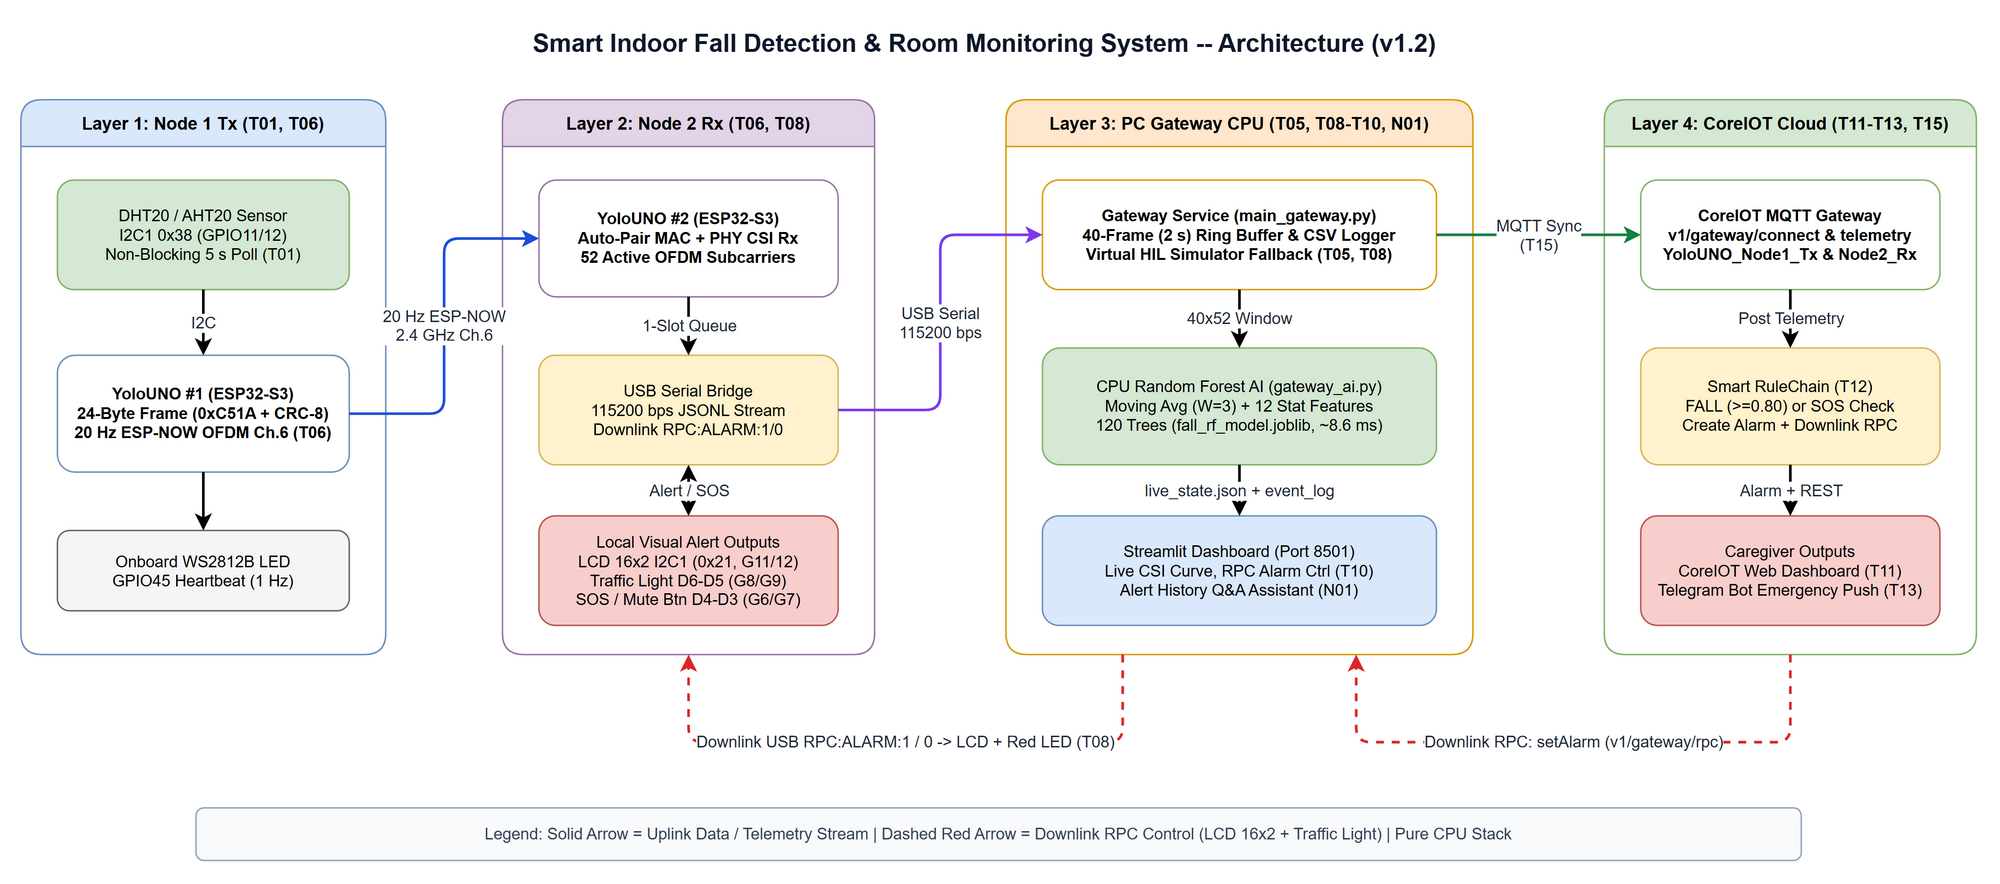
\includegraphics[width=0.98\textwidth]{graphics/v1_2_drawio_overall_architecture.png}
\caption{Overall Four-Layer Architecture of the Smart Fall Detection System with Verified Grove Hardware Visual Alerting (v1.2)}
\label{fig:overall_arch}
\end{figure}

Data flows cleanly across the four layers:
\begin{enumerate}
  \item \textbf{Layer 1 -- Node~1 Transmitter \& Environment (\texttt{YoloUNO \#1}):} Reads ambient temperature and humidity from the I2C \texttt{DHT20} sensor (\texttt{I2C1}, \texttt{0x38}) every 5~seconds using a non-blocking state machine, packs them into a 24-byte binary frame with magic header \texttt{0xC51A} and CRC-8 checksum, and transmits at a steady \textbf{20~Hz} (50~ms period) over Wi-Fi Channel~6 using IEEE~802.11n OFDM (\texttt{WIFI\_PHY\_RATE\_MCS0\_LGI}) via ESP-NOW.
  \item \textbf{Layer 2 -- Node~2 CSI Receiver \& Grove Visual Alert (\texttt{YoloUNO \#2}):} Auto-pairs with Node~1, captures the 64-subcarrier PHY-layer CSI array inside an IRAM interrupt callback, extracts 52 active OFDM subcarrier amplitudes, and streams newline-delimited JSON (\texttt{JSONL}) at \textbf{115200~bps} over USB Serial to the PC Gateway while monitoring the Grove \texttt{D4--D3} (\texttt{GPIO6/7}) SOS button and executing downlink \texttt{RPC:ALARM:1/0} and \texttt{RPC:STATE:*} commands to drive the \textbf{OhStem LCD~16x2 I2C display} (\texttt{I2C1 0x21}) and \textbf{2-bit Traffic Light LED module} (\texttt{D6--D5}, \texttt{GPIO8/9}).
  \item \textbf{Layer 3 -- PC Local IoT Gateway (Pure CPU):} Maintains a 40-frame (2.0-second) sliding buffer (or connects seamlessly to the built-in \texttt{VirtualYoloUnoCluster} simulator when hardware is unplugged), computes 3-frame Moving Average smoothing and 12 statistical features every 5 frames (0.25~s stride), runs the 120-tree \texttt{scikit-learn} Random Forest classifier, writes atomic live snapshots to \texttt{live\_state.json}, logs critical alerts to \texttt{event\_log.jsonl}, and serves the Streamlit real-time dashboard and \texttt{N01} Assistant on port \texttt{8501}.
  \item \textbf{Layer 4 -- CoreIOT Cloud \& Telegram Alerting:} Synchronizes both virtual child devices (\texttt{YoloUNO\_Node1\_Tx} and \texttt{YoloUNO\_Node2\_Rx}) over standard ThingsBoard/CoreIOT MQTT Gateway topics (\texttt{v1/gateway/connect}, \texttt{telemetry}, \texttt{attributes}, \texttt{rpc}), evaluates the 7-node \texttt{Smart\_Room\_Fall\_Alert\_RuleChain}, displays remote widgets, pushes emergency alerts via Telegram Bot REST API, and sends remote \texttt{setAlarm} RPC commands back down to Node~2's LCD~16x2 and Red Traffic Light indicator.
\end{enumerate}

\subsection{Functional Decomposition}
Figure~\ref{fig:func_decomp} decomposes the v1.2 system into four cohesive subsystems aligned directly with the three-member team structure. Each subsystem exposes a well-defined interface (I2C, 24-byte ESP-NOW, 115200~bps JSONL Serial, and CoreIOT MQTT JSON), enabling independent testing and modular peripheral swaps on Node~2 without altering the AI or Cloud layers.

\begin{figure}[H]
\centering
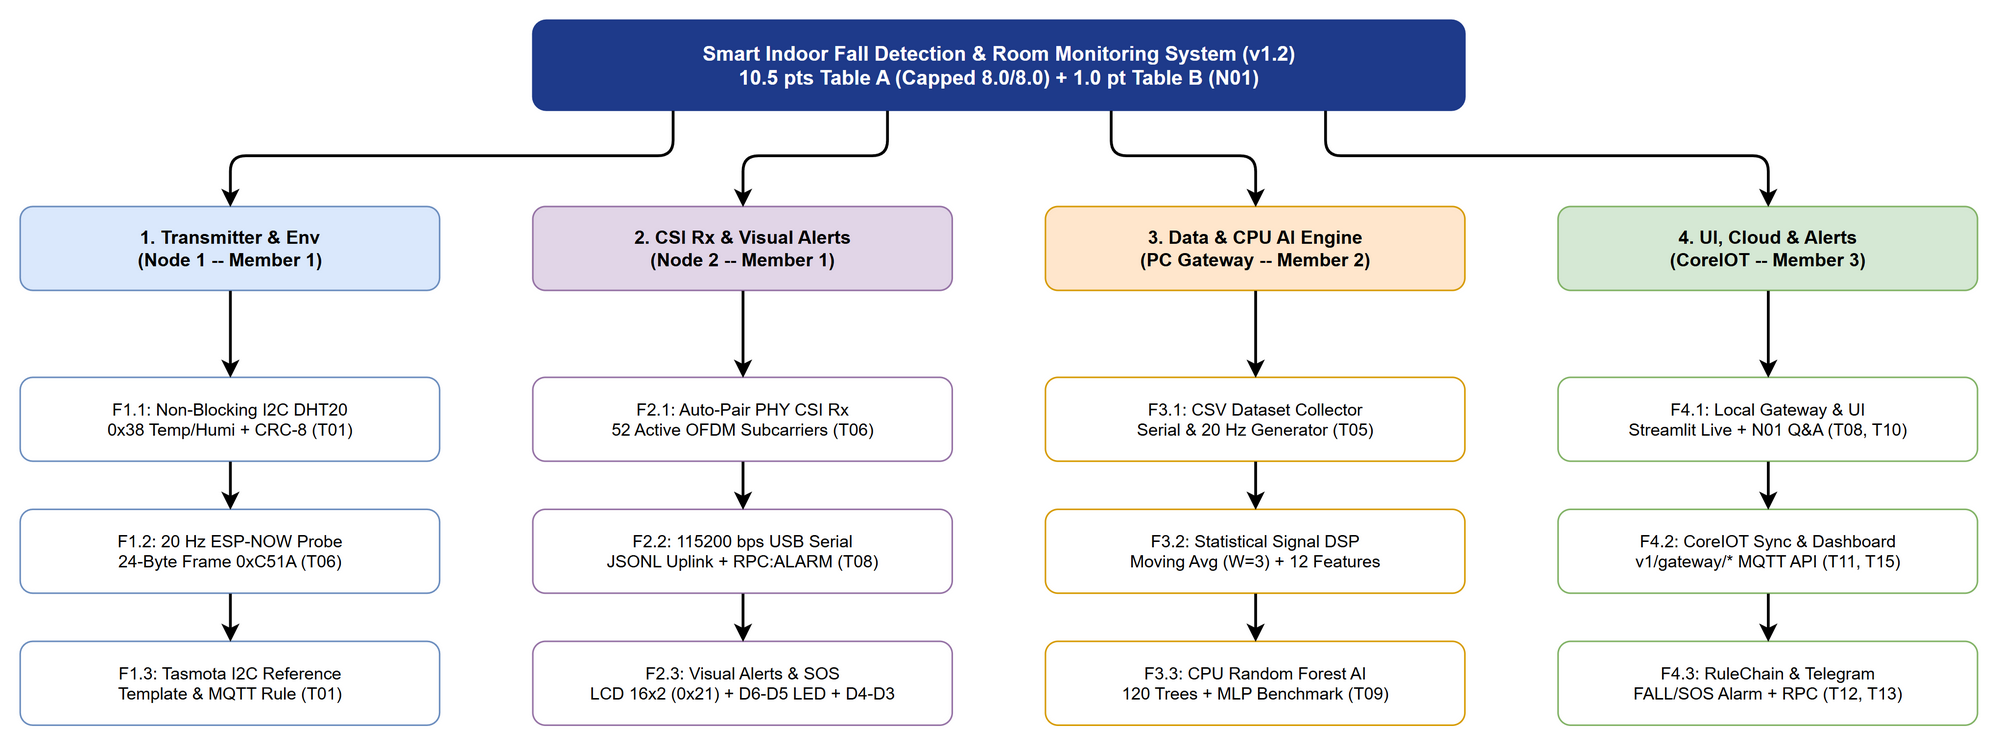
\includegraphics[width=0.96\textwidth]{graphics/v1_2_drawio_functional_decomposition.png}
\caption{Functional Decomposition Across Four Subsystems and Team Responsibilities (v1.2)}
\label{fig:func_decomp}
\end{figure}

\subsection{Feature Layer Analysis and Architectural Evolution (v1.0 $\rightarrow$ v1.2)}
A major engineering lesson across iterations was balancing academic ambition against physical lab availability and system stability. Table~\ref{tab:streamlining_rationale} summarizes both the v1.1 software/RF streamlining and the v1.2 Node~2 Grove visual-alert upgrade.

\begin{table}[H]
\centering
\caption{Engineering Rationale Behind Architectural Evolution from v1.0 to v1.2}
\label{tab:streamlining_rationale}
\footnotesize
\begin{tabularx}{\textwidth}{|P{2.7cm}|P{3.6cm}|P{3.8cm}|Y|}
\hline
\textbf{Subsystem} & \textbf{Previous Design (v1.0 / v1.1)} & \textbf{Current v1.2 Design} & \textbf{Concrete Engineering Benefit} \\
\hline
RF Link \& Serial Rate & 100~Hz ESP-NOW + 921600~bps USB-CDC (v1.0) & 20~Hz ESP-NOW + 115200~bps USB Serial & 5$\times$ lower packet pressure; eliminates USB UART drops while preserving 0--10~Hz Nyquist band for falls. \\
\hline
Signal Processing (DSP) & Hampel + 4th-order Butterworth SOS + STFT (v1.0) & 3-frame Moving Average + 12 basic statistics & Transparent math (\texttt{Std}, \texttt{Max-Min}, \texttt{Peak/Tail}); zero \texttt{scipy} dependency; easy to explain. \\
\hline
AI Inference Stack & ESP32 INT8 1D-CNN + RTX~5070 CUDA 2D-CNN (v1.0) & Single \texttt{scikit-learn} Random Forest (CPU, 585~KB) & Runs on any Windows/macOS/Linux laptop in $\approx 8.6\text{ ms}$ without PyTorch, ONNX, or NVIDIA CUDA. \\
\hline
Node~2 MCU Scope & CSI + BLE + TinyML + HTTP Web + OTA (v1.0) & CSI capture + Serial bridge + I2C LCD/Traffic Light/SOS + Auto-Pair & Eliminates Wi-Fi/BLE antenna coexistence drops, memory pressure, and manual MAC hardcoding. \\
\hline
Node~2 Alert Peripherals & KY-012 Buzzer (\texttt{GPIO10}) + WS2812B (\texttt{GPIO18}) (v1.1) & \textbf{LCD~16x2 (\texttt{I2C1 0x21}) + Traffic Light (\texttt{D6--D5}) + Btn (\texttt{D4--D3})} & Plug-and-play OhStem Grove cables (zero loose jumpers); live text (Temp/Humi/State) + intuitive 2-bit R/Y/G indicator. \\
\hline
Table~B Bonus Feature & GPU CUDA (\texttt{N04}) + STFT Snapshots (\texttt{N06}) (v1.0) & Alert History Q\&A Assistant (\texttt{N01}) & Deterministic, fast, verifiable on CPU, and earns full 1.0/1.0 credit in Table~B. \\
\hline
\end{tabularx}
\end{table}

\subsection{Feature -- Technology Element Mapping}
Table~\ref{tab:feat_tech_map} traces every user-facing feature in v1.2 to its exact course technology code and software/firmware module.

\begin{table}[H]
\centering
\caption{Traceability Matrix Linking System Features to Course Technology Codes (v1.2)}
\label{tab:feat_tech_map}
\footnotesize
\begin{tabularx}{\textwidth}{|P{3.4cm}|C{1.4cm}|P{4.4cm}|Y|}
\hline
\textbf{User-Facing Feature} & \textbf{Tech Code} & \textbf{Primary Implementation File} & \textbf{Verification Mechanism} \\
\hline
Ambient Room Temp \& Humidity Monitoring & \texttt{T01} & \texttt{firmware/\allowbreak node1\_tx\_env/\allowbreak src/\allowbreak main.cpp} & Non-blocking I2C \texttt{0x38} read + CRC-8 (\texttt{0x31}) + Tasmota template guide \\
\hline
20~Hz Camera-Free Wi-Fi CSI Sensing Link & \texttt{T06} & \texttt{firmware/\allowbreak include/\allowbreak csi\_protocol.h}, \texttt{node2\_rx\_csi} & 24-byte \texttt{0xC51A} CRC-8 C++17 unit test + Auto-Pair MAC lock \\
\hline
Labeled 20~Hz CSI Dataset Recording & \texttt{T05} & \texttt{ai\_training/\allowbreak csi\_serial\_\allowbreak collector.py} & Generates clean 52-subcarrier CSV files from USB Serial or Simulator \\
\hline
Real-Time Local Ingestion \& Visual Alert RPC & \texttt{T08} & \texttt{gateway/\allowbreak main\_gateway.py} & 40-frame ring buffer + downlink \texttt{RPC:ALARM:1/0} to I2C LCD~16x2 \& Traffic Light \\
\hline
Pure-CPU Fall Classification AI & \texttt{T09} & \texttt{gateway/\allowbreak gateway\_ai.py}, \texttt{train\_gateway\_\allowbreak ai.py} & 99.58\% test accuracy, 100\% Fall F1, 8.60~ms mean CPU latency \\
\hline
Live Disturbance Chart \& Control Portal & \texttt{T10} & \texttt{gateway/\allowbreak streamlit\_ui.py} & Interactive Plotly curves, KPI cards, scenario injector, RPC buttons \\
\hline
Remote Cloud Dashboard \& Device Sync & \texttt{T11}, \texttt{T15} & \texttt{coreiot/\allowbreak dashboard\_\allowbreak template.json}, \texttt{coreiot\_\allowbreak sync.py} & Standard \texttt{v1/gateway/connect}, \texttt{telemetry}, \texttt{attributes}, \texttt{rpc} MQTT \\
\hline
Automated Cloud Fall/SOS Alerting & \texttt{T12}, \texttt{T13} & \texttt{coreiot/\allowbreak rulechain\_\allowbreak fall.json}, \texttt{coreiot\_\allowbreak sync.py} & 7-node RuleChain + Telegram Bot REST API with 15~s cooldown \\
\hline
Natural-Language Alert History Assistant & \texttt{N01} & \texttt{gateway/\allowbreak streamlit\_ui.py} (Tab~2) & Queries \texttt{event\_log.jsonl} for fall counts, latest alert, SOS, and temp/humi \\
\hline
\end{tabularx}
\end{table}

\subsection{New Technologies Beyond Standard Lectures}
Beyond core IoT lecture topics (I2C sensors, MQTT, and ThingsBoard/CoreIOT dashboards), our v1.2 project integrates three practical engineering techniques:
\begin{enumerate}
  \item \textbf{IEEE 802.11n PHY-Layer Wi-Fi CSI Extraction:} Accessing complex channel frequency responses across 52 active OFDM subcarriers via \texttt{esp\_wifi\_set\_csi\_rx\_cb()} to turn standard ESP32-S3 communication hardware into a passive RF motion sensor.
  \item \textbf{Temporal Surge-to-Stillness Feature Engineering:} Distinguishing real human falls from fast sitting (\texttt{sit\_fast} hard negatives) and continuous walking using interpretable time-split ratios (\texttt{peak\_to\_tail\_ratio} and \texttt{post\_peak\_std}) rather than opaque black-box deep networks.
  \item \textbf{Dual-Mode Hardware-in-the-Loop (HIL) Gateway \& Plug-and-Play Grove Hardware:} Running the exact same \texttt{LocalIoTGatewayService}, Random Forest engine, CoreIOT MQTT synchronizer, and Streamlit UI across live USB Serial hardware (featuring verified Grove LCD~16x2 \texttt{0x21}, Traffic Light \texttt{D6--D5}, and SOS button \texttt{D4--D3}) and a deterministic virtual simulator via a single YAML key (\texttt{source\_mode}).
\end{enumerate}

\subsection{Hardware List and Bill of Materials}
Table~\ref{tab:bom} presents the updated Bill of Materials (BOM) for the v1.2 hardware setup. Replacing the active buzzer and raw WS2812B LED strip with OhStem Grove modules (LCD~16x2 I2C \texttt{0x21} on \texttt{I2C1} and 2-bit Traffic Light LED on \texttt{D6--D5}) increases total hardware cost by only 60,000~VND ($\approx$ \$2.4~USD) while providing plug-and-play Grove connectivity and clear text/color feedback during live classroom demos.

\begin{table}[H]
\centering
\caption{Hardware Components and Estimated Bill of Materials (v1.2)}
\label{tab:bom}
\footnotesize
\begin{tabularx}{\textwidth}{|C{0.7cm}|P{3.8cm}|C{0.8cm}|P{3.6cm}|R{2.1cm}|Y|}
\hline
\textbf{No.} & \textbf{Component Name} & \textbf{Qty} & \textbf{Key Specification} & \textbf{Cost (VND)} & \textbf{Assigned Role} \\
\hline
1 & OhStem YoloUNO (ESP32-S3) & 2 & Dual-core 240~MHz, Wi-Fi 802.11n CSI, 2$\times$ Grove I2C & 360,000 & Node~1 Tx \& Node~2 CSI Rx \\
\hline
2 & DHT20 / AHT20 I2C Module & 1 & I2C \texttt{0x38}, $\pm 0.5^\circ$C, $\pm 3\%$RH, 3.3~V & 45,000 & Room environmental sensor (\texttt{T01}) \\
\hline
3 & \textbf{OhStem LCD~16x2 I2C Module} & 1 & 16$\times$2 char LCD, PCF8574 \texttt{0x21} (Grove \texttt{I2C1}) & 55,000 & Live room status, Temp/Humi \& flashing \texttt{FALL ALERT} text \\
\hline
4 & \textbf{Grove Traffic Light LED Module} & 1 & 3-LED R/Y/G 2-bit module (Grove \texttt{D6--D5}) & 45,000 & Visual beacon (Green=Safe, Yellow=Walk, Red=Alert) \\
\hline
5 & Grove Push Button Module & 1 & Dual/Single button (\texttt{INPUT\_PULLUP}, \texttt{D4--D3}) & 5,000 & 3~s SOS trigger / short-tap mute \\
\hline
6 & USB-C \& 4-Pin Grove Cables & 2 & 1$\times$ 5~V Power + 1$\times$ Data USB-C + 3$\times$ Grove I2C & 60,000 & Node~1 power, Node~2 Serial \& I2C bus wiring \\
\hline
7 & Standard Student Laptop & 1 & Any CPU (Windows/Linux/macOS) & Existing & PC Gateway, CPU AI, Streamlit UI \\
\hline
\multicolumn{4}{|r|}{\textbf{Total Estimated Hardware Cost (Excluding Existing Laptop)}} & \textbf{570,000} & \textbf{$\approx$ 23~USD complete 2-node kit} \\
\hline
\end{tabularx}
\end{table}

% =========================================================================
% CHAPTER 3: SYSTEM IMPLEMENTATION
% =========================================================================
\section{System Implementation}

\subsection{Hardware and Wiring Diagrams}
Figure~\ref{fig:hw_wiring} illustrates the complete v1.2 electrical interconnection of Node~1 (\texttt{YoloUNO \#1}) and Node~2 (\texttt{YoloUNO \#2}), while Tables~\ref{tab:pin_node1} and~\ref{tab:pin_node2} specify exact GPIO pin assignments reflecting OhStem YoloUNO's onboard Grove I2C headers and \texttt{firmware/include/config.example.h}.

\begin{figure}[H]
\centering
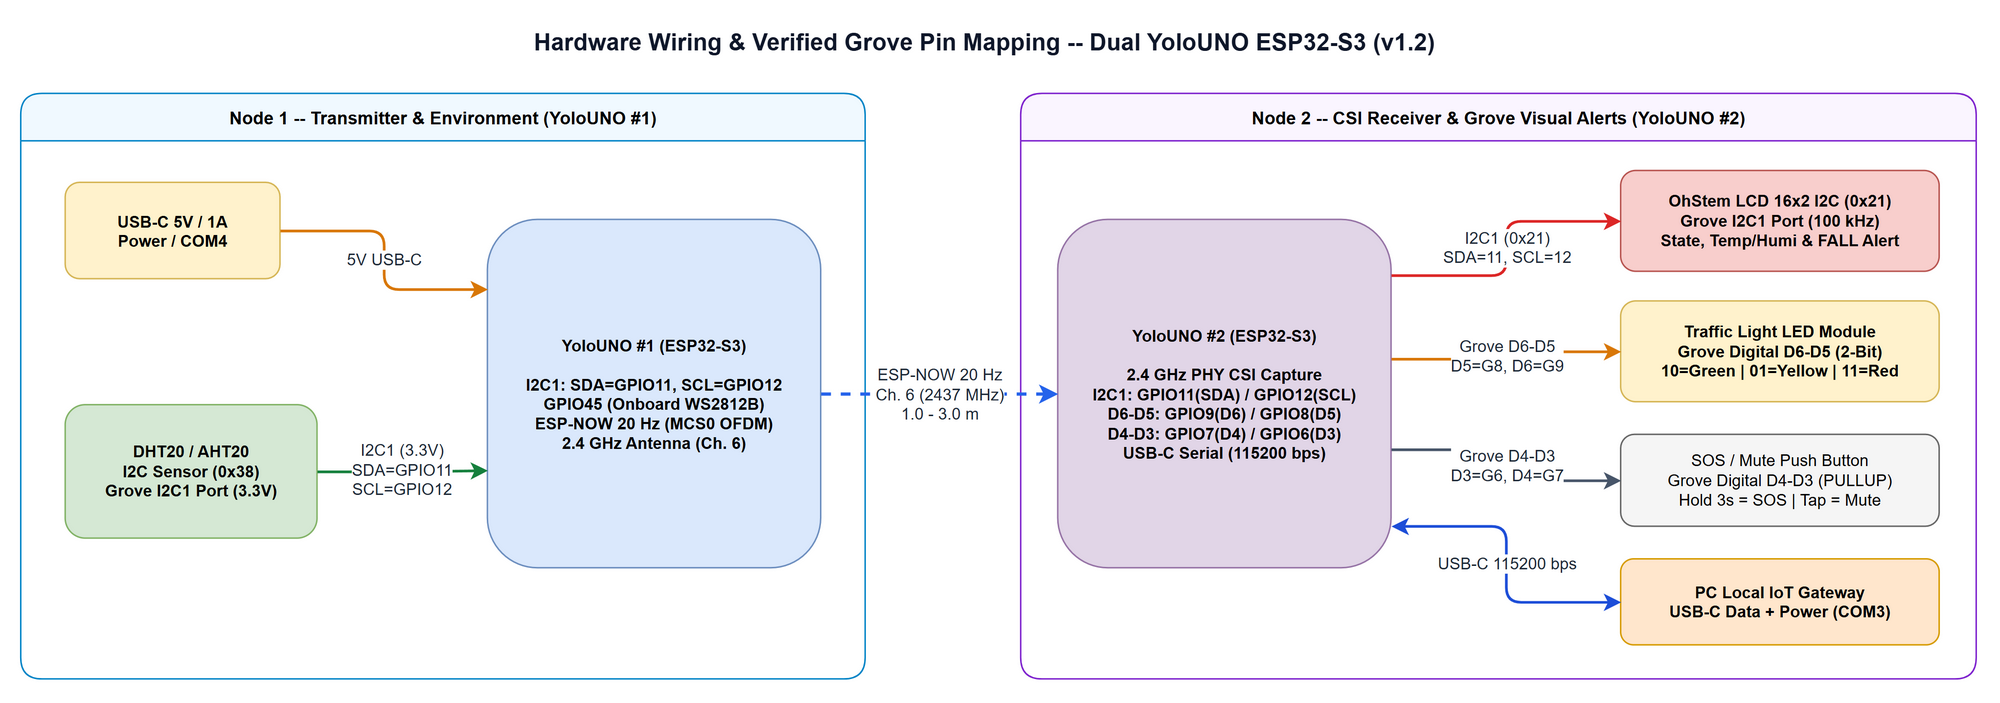
\includegraphics[width=0.98\textwidth]{graphics/v1_2_drawio_hardware_wiring.png}
\caption{Hardware Wiring and Verified Grove Pin Mapping for Dual YoloUNO (ESP32-S3) Boards (v1.2)}
\label{fig:hw_wiring}
\end{figure}

\begin{table}[H]
\centering
\caption{Node~1 (\texttt{YoloUNO \#1} -- Transmitter \& I2C DHT20) Verified GPIO Pin Map (v1.2)}
\label{tab:pin_node1}
\footnotesize
\begin{tabularx}{\textwidth}{|P{3.0cm}|C{2.4cm}|C{2.6cm}|Y|}
\hline
\textbf{Peripheral} & \textbf{Grove Port} & \textbf{ESP32-S3 Pin} & \textbf{Electrical / Protocol Configuration} \\
\hline
DHT20 / AHT20 & \texttt{I2C1} (\texttt{3V3/GND}) & \texttt{3V3} / \texttt{GND} & Regulated 3.3~V supply rail (Grove \texttt{I2C1}) \\
\hline
DHT20 / AHT20 & \texttt{I2C1} (\texttt{SDA}) & \texttt{GPIO11} & I2C data line, 100~kHz standard mode (\texttt{0x38}) \\
\hline
DHT20 / AHT20 & \texttt{I2C1} (\texttt{SCL}) & \texttt{GPIO12} & I2C clock line, 100~kHz standard mode (\texttt{0x38}) \\
\hline
Onboard RGB LED & Onboard & \texttt{GPIO45} & Onboard WS2812B heartbeat blinking at 1~Hz \\
\hline
Power Input & \texttt{USB-C} & \texttt{5V USB-C} & 5~V / 1~A adapter or PC USB (\texttt{COM4} during bring-up) \\
\hline
\end{tabularx}
\end{table}

\begin{table}[H]
\centering
\caption{Node~2 (\texttt{YoloUNO \#2} -- CSI Receiver, USB Bridge \& Grove Visual Alert) Verified GPIO Pin Map (v1.2)}
\label{tab:pin_node2}
\footnotesize
\begin{tabularx}{\textwidth}{|P{3.1cm}|C{2.4cm}|C{2.7cm}|Y|}
\hline
\textbf{Peripheral} & \textbf{Grove Port} & \textbf{ESP32-S3 Pin} & \textbf{Electrical / Protocol Configuration} \\
\hline
\textbf{OhStem LCD~16x2 I2C} & \texttt{I2C1}\newline(\texttt{SDA/SCL}) & \texttt{GPIO11} / \texttt{GPIO12} & Hardware I2C0 (100~kHz, verified addr \texttt{0x21}); 2-line room status \& blinking \texttt{!! FALL ALERT !!} \\
\hline
\textbf{Traffic Light LED} & \texttt{D6--D5}\newline(\texttt{D5/D6}) & \texttt{GPIO8} / \texttt{GPIO9} & 2-bit digital output: \texttt{(1,0)}=Green, \texttt{(0,1)}=Yellow, \texttt{(1,1)}=Red, \texttt{(0,0)}=Off \\
\hline
\textbf{SOS / Mute Button} & \texttt{D4--D3}\newline(\texttt{D3/D4}) & \texttt{GPIO6} / \texttt{GPIO7} & Internal \texttt{INPUT\_PULLUP} (idle \texttt{HIGH}); hold $\geq 3\text{ s}$ triggers SOS, short tap clears alert \\
\hline
Onboard LED Mirror & Onboard & \texttt{GPIO45} / \texttt{GPIO48} & Onboard NeoPixel + \texttt{LED\_BUILTIN} mirror alarm state \\
\hline
PC Gateway Link & \texttt{USB-C} & \texttt{USB-C} (\texttt{COM3}) & Bidirectional 115200~bps JSONL uplink + \texttt{RPC:ALARM}/\texttt{RPC:STATE} downlink \\
\hline
\end{tabularx}
\end{table}

\noindent\textbf{Official OhStem YoloUNO Pin Mapping Verification:} Using OhStem's official \texttt{ohstem\_esp32-3.1.3/variants/yolo\_uno/pins\_arduino.h} definition, the white Grove Digital ports map directly to ESP32-S3 GPIOs (\texttt{D3 = GPIO6}, \texttt{D4 = GPIO7}, \texttt{D5 = GPIO8}, \texttt{D6 = GPIO9}), while the red Grove \texttt{I2C1} port maps to \texttt{SDA = GPIO11} and \texttt{SCL = GPIO12}. An on-board I2C scan on Node~2 verified the OhStem LCD~16x2 backpack at address \texttt{0x21} (decimal~33, matching HCMUT Lab~3), while physical bench testing confirmed both the 2-bit Traffic Light module on \texttt{D6--D5} and the push-button module on \texttt{D4--D3}.

\subsection{Device Firmware Implementation}
Figure~\ref{fig:fw_arch} depicts the streamlined v1.2 firmware execution flow for both boards. Both firmware sketches avoid complex multi-core manual spinlocks, eliminate blocking sensor delays, and include preprocessor guards (\texttt{ESP\_ARDUINO\_VERSION\_MAJOR >= 3}) so they compile cleanly across both Arduino-ESP32 v2.x and v3.x toolchains.

\begin{figure}[H]
\centering
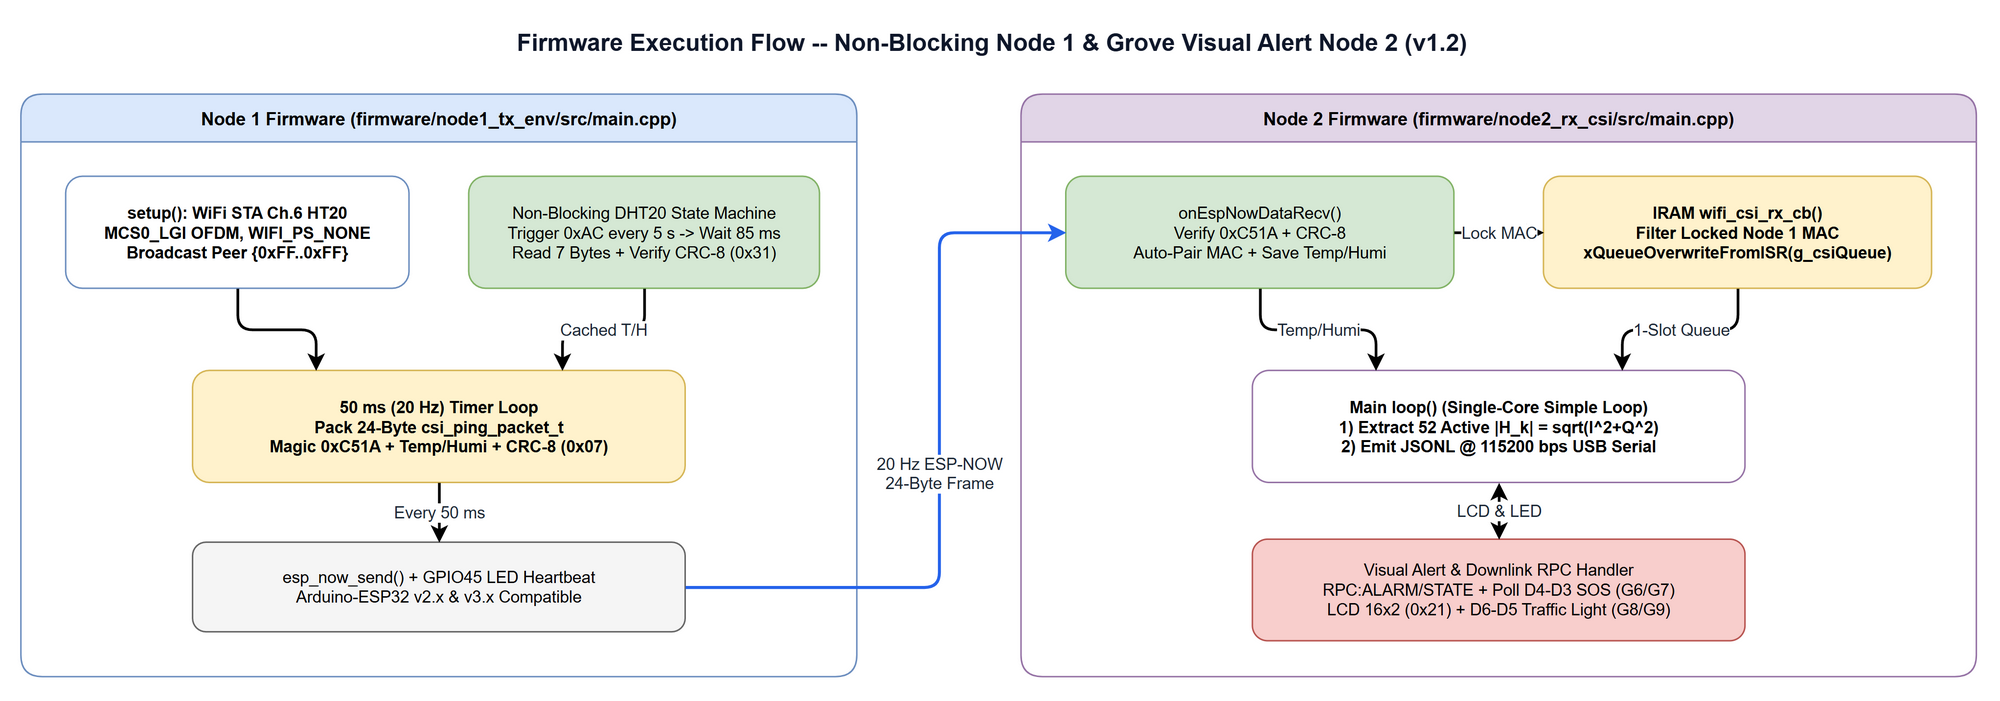
\includegraphics[width=0.98\textwidth]{graphics/v1_2_drawio_firmware_architecture.png}
\caption{Streamlined Firmware Execution Flow: Non-Blocking Node~1 and Auto-Pair Grove Alert Node~2 (v1.2)}
\label{fig:fw_arch}
\end{figure}

\subsubsection{Node~1 Firmware: Non-Blocking I2C DHT20 and 20~Hz ESP-NOW (\texttt{T01}, \texttt{T06})}
In \texttt{firmware/node1\_tx\_env/src/main.cpp}, the DHT20 sensor driver implements a lightweight two-state non-blocking cycle inside \texttt{loop()}:
\begin{enumerate}
  \item Every 5000~ms, Node~1 issues the I2C trigger sequence \texttt{0xAC 0x33 0x00} to address \texttt{0x38} and sets \texttt{g\_dhtWaitingAdc = true}, immediately returning so the 20~Hz ESP-NOW timer never stalls.
  \item Once 85~ms has elapsed, Node~1 reads 7 bytes, checks the busy bit (\texttt{raw[0] \& 0x80 == 0}), verifies the Aosong CRC-8 checksum (polynomial \texttt{0x31}, initial value \texttt{0xFF}), and converts the 20-bit raw humidity and temperature registers into floating-point \texttt{g\_latestHumiRh} and \texttt{g\_latestTempC}.
\end{enumerate}
In parallel, we document the exact \textbf{Tasmota ESP32-S3} configuration template (\texttt{GPIO11 = I2C SDA (640)}, \texttt{GPIO12 = I2C SCL (608)}) and MQTT \texttt{Rule1} commands in \texttt{firmware/node1\_tx\_env/tasmota\_yolo\_uno\_dht20.md} to directly demonstrate \texttt{T01}.

Every 50~ms (\textbf{20~Hz}), Node~1 packs the latest temperature, humidity, sequence counter, status bitmask, and CRC-8 checksum into \texttt{csi\_ping\_packet\_t}, toggles its onboard \texttt{GPIO45} RGB heartbeat once per second, and calls \texttt{esp\_now\_send()} on Channel~6 with \texttt{esp\_wifi\_config\_espnow\_rate(WIFI\_IF\_STA, WIFI\_PHY\_RATE\_MCS0\_LGI)} so every packet uses IEEE~802.11n HT20 OFDM modulation (generating 64-subcarrier LLTF CSI frames rather than legacy 1~Mbps 802.11b DSSS).

\subsubsection{Node~2 Firmware: Auto-Pair CSI Capture and Grove Visual Alerts (\texttt{T06}, \texttt{T08})}
In \texttt{firmware/node2\_rx\_csi/src/main.cpp}, Node~2 configures \texttt{WIFI\_STA} on Channel~6 with hardware CSI enabled (\texttt{lltf\_en = true}, \texttt{channel\_filter\_en = true}) \emph{first}, and then initializes its PCF8574 I2C LCD~16x2 (\texttt{0x21} on \texttt{GPIO11/12}) once the 3.3~V rail settles after Wi-Fi RF calibration:
\begin{itemize}
  \item \textbf{Plug-and-Play Auto-Pair:} When \texttt{NODE1\_TX\_MAC\_ADDR} is left as broadcast \texttt{\{0xFF, ..., 0xFF\}}, the ESP-NOW receive callback \texttt{onEspNowDataRecv()} verifies magic header \texttt{0xC51A} and CRC-8 (\texttt{0x07}), automatically learns Node~1's real MAC address, and sets \texttt{g\_targetMacLocked = true}.
  \item \textbf{Zero-Lock ISR Queue:} The IRAM PHY callback \texttt{wifi\_csi\_rx\_cb()} filters packets matching \texttt{g\_targetNode1Mac} and writes the 128-byte raw I/Q buffer into a 1-slot FreeRTOS queue using \texttt{xQueueOverwriteFromISR()}, guaranteeing the main loop always receives the freshest frame without race conditions or backlog lag.
  \item \textbf{USB Serial Uplink \& Grove Visual Output:} The main \texttt{loop()} converts the 128-byte I/Q array into 52 active subcarrier amplitudes $|H_k| = \sqrt{I_k^2 + Q_k^2}$, emits a single JSONL line at 115200~bps, polls the Grove \texttt{D4--D3} (\texttt{GPIO6/7}) SOS/Mute button (auto-learning its resting logic level at boot), and executes downlink \texttt{RPC:ALARM:1/0} and \texttt{RPC:STATE:*} commands from the PC Gateway to update the OhStem LCD~16x2 (\texttt{0x21}) and 2-bit Traffic Light LED module (\texttt{D6--D5}, \texttt{GPIO8/9}) according to Table~\ref{tab:node2_visual_states}. Refreshing the LCD only on string change keeps I2C bus occupancy negligible so the 20~Hz CSI serial uplink never stalls.
\end{itemize}

\begin{table}[H]
\centering
\caption{Node~2 Verified Hardware Visual State Mapping (LCD~16x2 \texttt{0x21} + Traffic Light \texttt{D6--D5}, v1.2)}
\label{tab:node2_visual_states}
\footnotesize
\renewcommand{\arraystretch}{1.08}
\begin{tabularx}{\textwidth}{|P{2.8cm}|C{2.7cm}|P{3.6cm}|Y|}
\hline
\textbf{System State / Trigger} & \textbf{Traffic Light (\texttt{D5, D6})} & \textbf{LCD~16x2 Line 1 (16 chars)} & \textbf{LCD~16x2 Line 2 \& Backlight Behavior} \\
\hline
\texttt{EMPTY} / \texttt{STATIONARY} & \textbf{Green} \texttt{(1, 0)} Solid & \texttt{STATE: SAFE} & \texttt{T:26.4C H:52\%} (Steady backlight) \\
\hline
\texttt{WALKING} & \textbf{Yellow} \texttt{(0, 1)} Solid & \texttt{STATE: WALKING} & \texttt{T:26.4C H:52\%} (Steady backlight) \\
\hline
\texttt{FALL} / \texttt{RPC:ALARM:1} & \textbf{Red} \texttt{(1, 1)} Blink & \texttt{!! FALL ALERT !!} & \texttt{CHECK ROOM NOW!} (Backlight blink) \\
\hline
\texttt{SOS} (\texttt{D4--D3} Hold 3~s) & \textbf{Red} \texttt{(1, 1)} Blink & \texttt{!! SOS MANUAL !!} & \texttt{TAP BTN TO MUTE} (Backlight blink) \\
\hline
\end{tabularx}
\end{table}

\begin{lstlisting}[language=C++, basicstyle=\scriptsize\ttfamily, caption={Core PHY-Layer CSI Callback and 24-Byte Frame Definition (\texttt{csi\_protocol.h} \& \texttt{node2\_rx\_csi/src/main.cpp})}, label={lst:csi_protocol}]
#pragma pack(push, 1)
typedef struct {
  uint16_t magic_header;    // Fixed 0xC51A system packet signature
  uint32_t seq_id;          // Monotonic sequence ID for packet-loss tracking
  uint32_t tx_time_ms;      // Node 1 transmit timestamp (ms)
  float    temp_c;          // Room temperature from I2C DHT20 (T01)
  float    humi_rh;         // Relative humidity from I2C DHT20 (T01)
  uint8_t  tx_status_flag;  // Bit 0: DHT20_OK
  uint8_t  reserved_pad[4]; // Channel & Tx power metadata -> exact 24 bytes
  uint8_t  crc8_checksum;   // CRC-8 (poly 0x07) over first 23 bytes
} csi_ping_packet_t;
#pragma pack(pop)
static_assert(sizeof(csi_ping_packet_t) == 24, "Packet MUST be 24 bytes!");

static void IRAM_ATTR wifi_csi_rx_cb(void* /*ctx*/, wifi_csi_info_t* info) {
  if (!info || !info->buf || info->len < (int)CSI_RAW_IQ_BYTES) return;
  if (!g_targetMacLocked) return;
  if (memcmp(info->mac, g_targetNode1Mac, 6) != 0) return;

  csi_frame_t frame;
  frame.rssi = info->rx_ctrl.rssi;
  memcpy(frame.iq_raw, info->buf, CSI_RAW_IQ_BYTES);
  BaseType_t higherWoken = pdFALSE;
  xQueueOverwriteFromISR(g_csiQueue, &frame, &higherWoken);
  if (higherWoken == pdTRUE) portYIELD_FROM_ISR();
}
\end{lstlisting}

\subsection[Device-to-Device Communication (\texttt{T06})]{Device-to-Device Communication (\texttt{T06})}
Table~\ref{tab:espnow_frame} documents the byte-level layout of \texttt{csi\_ping\_packet\_t}, verified at compile time via \texttt{static\_assert(sizeof(csi\_ping\_packet\_t) == 24)} and at runtime by our host C++17 unit test (\texttt{tests/cpp\_protocol\_unit\_test.cpp}). At 20~Hz, the link consumes only $24 \times 20 = 480\text{ bytes/s}$ of payload bandwidth while triggering 20 clean IEEE 802.11n HT20 LLTF channel estimates per second. Excluding lower guard bands ($k \in [0,5]$), DC subcarrier ($k = 32$), and upper guard bands ($k \in [59,63]$) leaves exactly \textbf{52 active OFDM subcarriers} carrying indoor multipath motion energy.

\begin{table}[H]
\centering
\caption{Byte-Level Layout of the 24-Byte ESP-NOW CSI Probe Frame (\texttt{T06})}
\label{tab:espnow_frame}
\footnotesize
\begin{tabularx}{\textwidth}{|C{1.8cm}|P{3.0cm}|C{2.0cm}|Y|}
\hline
\textbf{Byte Offset} & \textbf{Field Name} & \textbf{C Type} & \textbf{Purpose and Integrity Check} \\
\hline
\texttt{[0..1]} & \texttt{magic\_header} & \texttt{uint16\_t} & Fixed constant \texttt{0xC51A} to reject unrelated 2.4~GHz frames \\
\hline
\texttt{[2..5]} & \texttt{seq\_id} & \texttt{uint32\_t} & Monotonic packet counter used by Node~2 to calculate \texttt{pkt\_loss\_pct} \\
\hline
\texttt{[6..9]} & \texttt{tx\_time\_ms} & \texttt{uint32\_t} & Node~1 uptime timestamp (\texttt{millis()}) for jitter monitoring \\
\hline
\texttt{[10..13]} & \texttt{temp\_c} & \texttt{float} & Latest I2C DHT20 ambient temperature ($^\circ$C) \\
\hline
\texttt{[14..17]} & \texttt{humi\_rh} & \texttt{float} & Latest I2C DHT20 relative humidity (\%RH) \\
\hline
\texttt{[18]} & \texttt{tx\_status\_flag} & \texttt{uint8\_t} & Bit~0 indicates valid live I2C DHT20 read vs.\ fallback \\
\hline
\texttt{[19..22]} & \texttt{reserved\_pad} & \texttt{uint8\_t[4]} & Channel index (6), Tx power indicator (+19.5~dBm), firmware version \\
\hline
\texttt{[23]} & \texttt{crc8\_checksum} & \texttt{uint8\_t} & SMBus/ITU-T CRC-8 (polynomial \texttt{0x07}) computed across bytes \texttt{[0..22]} \\
\hline
\end{tabularx}
\end{table}

\subsection[PC Local IoT Gateway and Dashboard (\texttt{T08}, \texttt{T10})]{PC Local IoT Gateway and Streamlit Dashboard (\texttt{T08}, \texttt{T10})}
The PC Local IoT Gateway (\texttt{gateway/main\_gateway.py}) bridges physical hardware (or the built-in \texttt{VirtualYoloUnoCluster} simulator) with the CPU Random Forest classifier, the local Streamlit dashboard, and CoreIOT Cloud:
\begin{itemize}
  \item \textbf{Dual Ingestion Modes:} In \texttt{serial} mode, \texttt{LocalIoTGatewayService} reads 115200~bps JSONL lines from \texttt{COM4}, appends each 52-subcarrier vector to a 40-frame ring buffer, and evaluates a new 2.0-second window every 5 frames (0.25~s stride). In \texttt{simulator} mode, it streams synthesized 40$\times$52 windows from \texttt{VirtualYoloUnoCluster} over local TCP (\texttt{127.0.0.1:19550}), enabling hardware-free demonstrations.
  \item \textbf{Bidirectional Downlink RPC:} Both CoreIOT remote RPC commands (\texttt{v1/gateway/rpc}) and local Streamlit button clicks (\texttt{ui\_commands.jsonl}) route through \texttt{handle\_downlink\_rpc()}, writing \texttt{RPC:ALARM:1\textbackslash n} or \texttt{RPC:ALARM:0\textbackslash n} to the USB Serial port to trigger or clear Node~2's I2C LCD~16x2 alert banner and Red Traffic Light LED (or updating the virtual simulator's alarm state).
  \item \textbf{Windows-Safe State Publishing:} Each inference cycle writes \texttt{live\_state.tmp} and atomically swaps it into \texttt{live\_state.json} with a short \texttt{PermissionError} retry loop so concurrent reads from Streamlit never crash the background gateway thread on Windows.
\end{itemize}

Figure~\ref{fig:streamlit_ui} shows a real live screenshot of the Streamlit Dashboard (\texttt{gateway/streamlit\_ui.py}) operating at \texttt{http://localhost:8501} during a triggered \texttt{FALL\_EMERGENCY} scenario: the left sidebar controls scenario selection, distance (1.0--3.5~m), through-wall NLOS toggle, and \texttt{Alarm ON} / \texttt{Mute Alarm} RPC buttons, while the main pane displays the red alert banner, four real-time KPI cards, the 2-second Moving-Average CSI disturbance curve, and the live Random Forest class probability bar chart (100.0\% \texttt{FALL} in 4.5~ms CPU).

\begin{figure}[H]
\centering
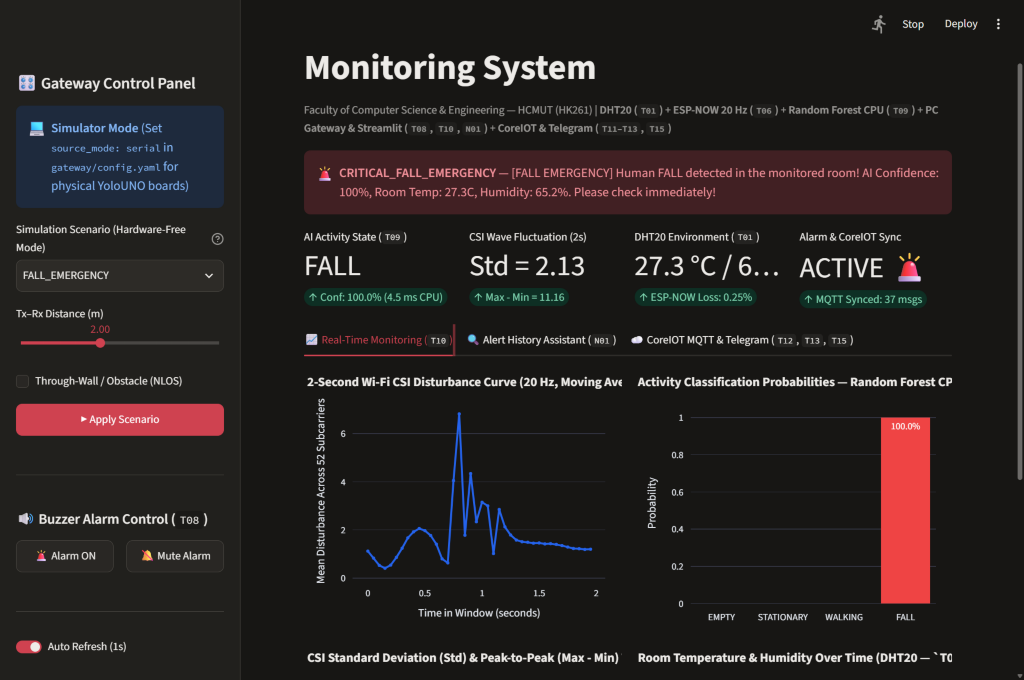
\includegraphics[width=0.96\textwidth]{graphics/v1_1_streamlit_live_fall.png}
\caption{Live Streamlit Gateway Dashboard (\texttt{T10}) Showing Triggered \texttt{FALL\_EMERGENCY}, 2-Second CSI Disturbance Spike, and 100.0\% CPU Random Forest Prediction}
\label{fig:streamlit_ui}
\end{figure}

\subsection[Artificial Intelligence Pipeline (\texttt{T05}, \texttt{T09})]{Artificial Intelligence Pipeline: Moving Average DSP \& CPU Random Forest (\texttt{T05}, \texttt{T09})}
Figure~\ref{fig:ai_pipeline} outlines the complete v1.2 data-collection, signal-processing, and classification pipeline implemented in \texttt{ai\_training/csi\_signal\_features.py}, \texttt{train\_gateway\_ai.py}, and \texttt{gateway/gateway\_ai.py}.

\begin{figure}[H]
\centering
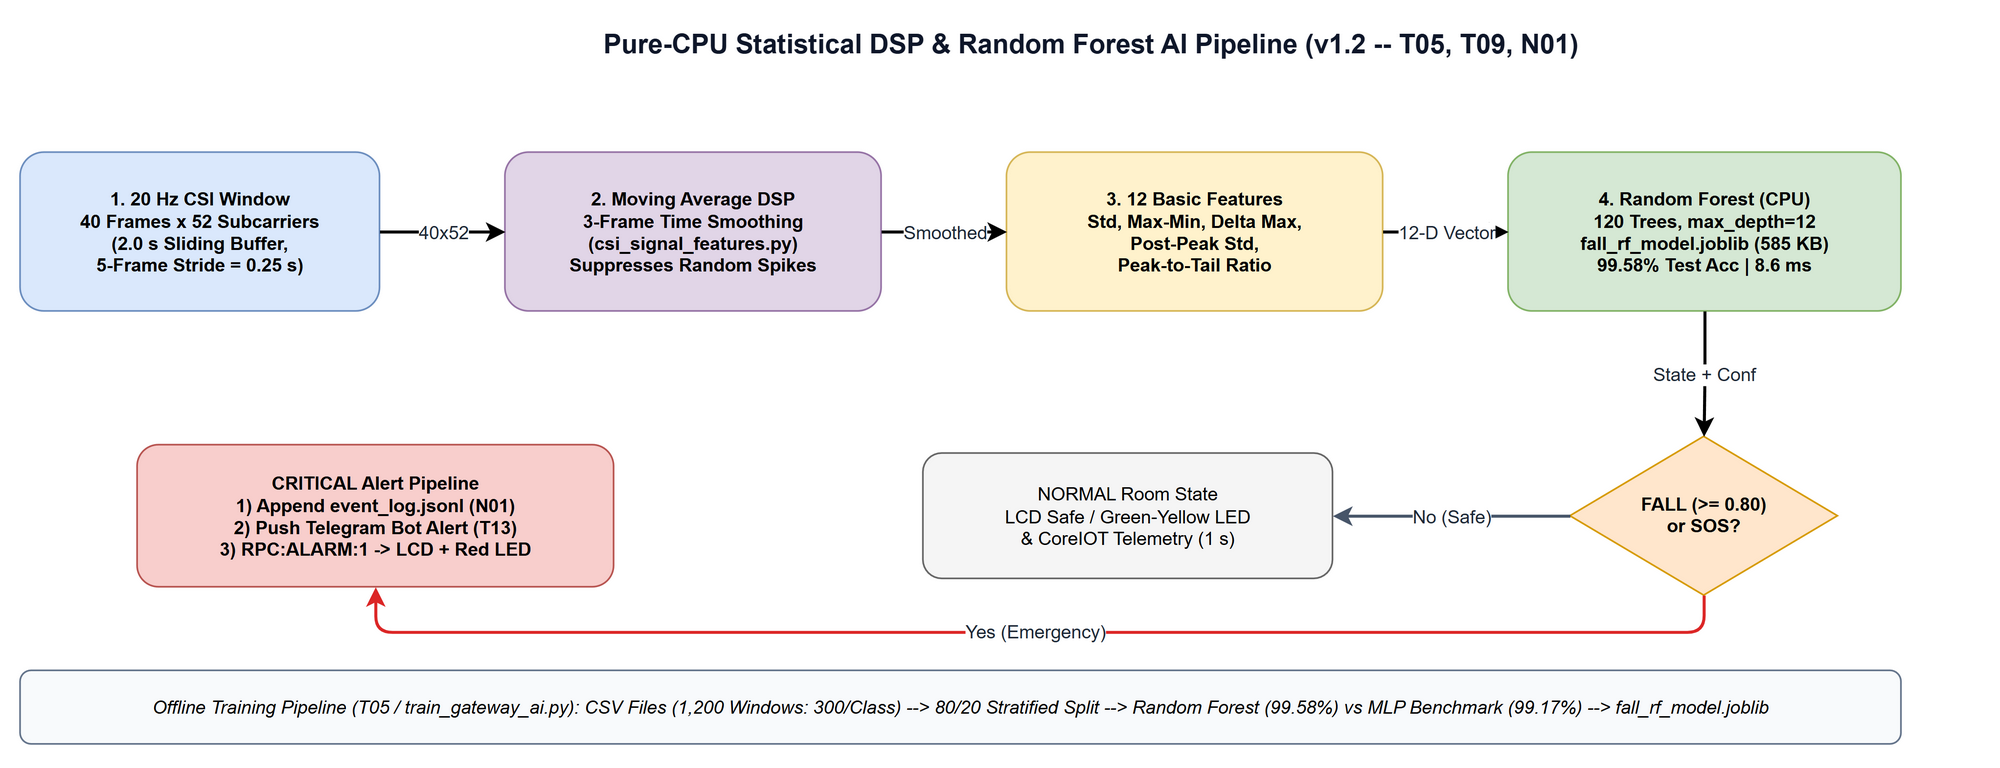
\includegraphics[width=0.98\textwidth]{graphics/v1_2_drawio_ai_pipeline.png}
\caption{Streamlined Pure-CPU Statistical DSP and Random Forest Classification Pipeline (v1.2)}
\label{fig:ai_pipeline}
\end{figure}

\subsubsection{Moving Average Smoothing and 12 Statistical Features}
Given a raw 2.0-second CSI amplitude matrix $A \in \mathbb{R}^{40 \times 52}$ sampled at $f_s = 20\text{ Hz}$, we first apply a 3-frame centered Moving Average along the time axis for each subcarrier $k \in \{0, \dots, 51\}$:
\begin{equation}
\tilde{A}_{t,k} = \frac{1}{3}\sum_{j=-1}^{1} A_{\text{clip}(t+j, 0, 39),\, k}
\label{eq:ma_smooth}
\end{equation}
Removing each subcarrier's per-window temporal median $\mu_k = \text{median}_t(\tilde{A}_{t,k})$ produces the zero-centered disturbance matrix $D_{t,k} = \tilde{A}_{t,k} - \mu_k$ and the 1-D room activity curve $c_t = \frac{1}{52}\sum_{k=0}^{51} |D_{t,k}|$ for $t = 0, \dots, 39$. Figure~\ref{fig:csi_four_classes} compares $c_t$ across all four activity classes: \texttt{EMPTY} remains flat near thermal noise, \texttt{STATIONARY} exhibits slow breathing ripples, \texttt{WALKING} oscillates continuously from 0.0~s to 2.0~s, and \texttt{FALL} displays an unmistakable sharp surge followed by abrupt post-impact floor stillness.

\begin{figure}[H]
\centering
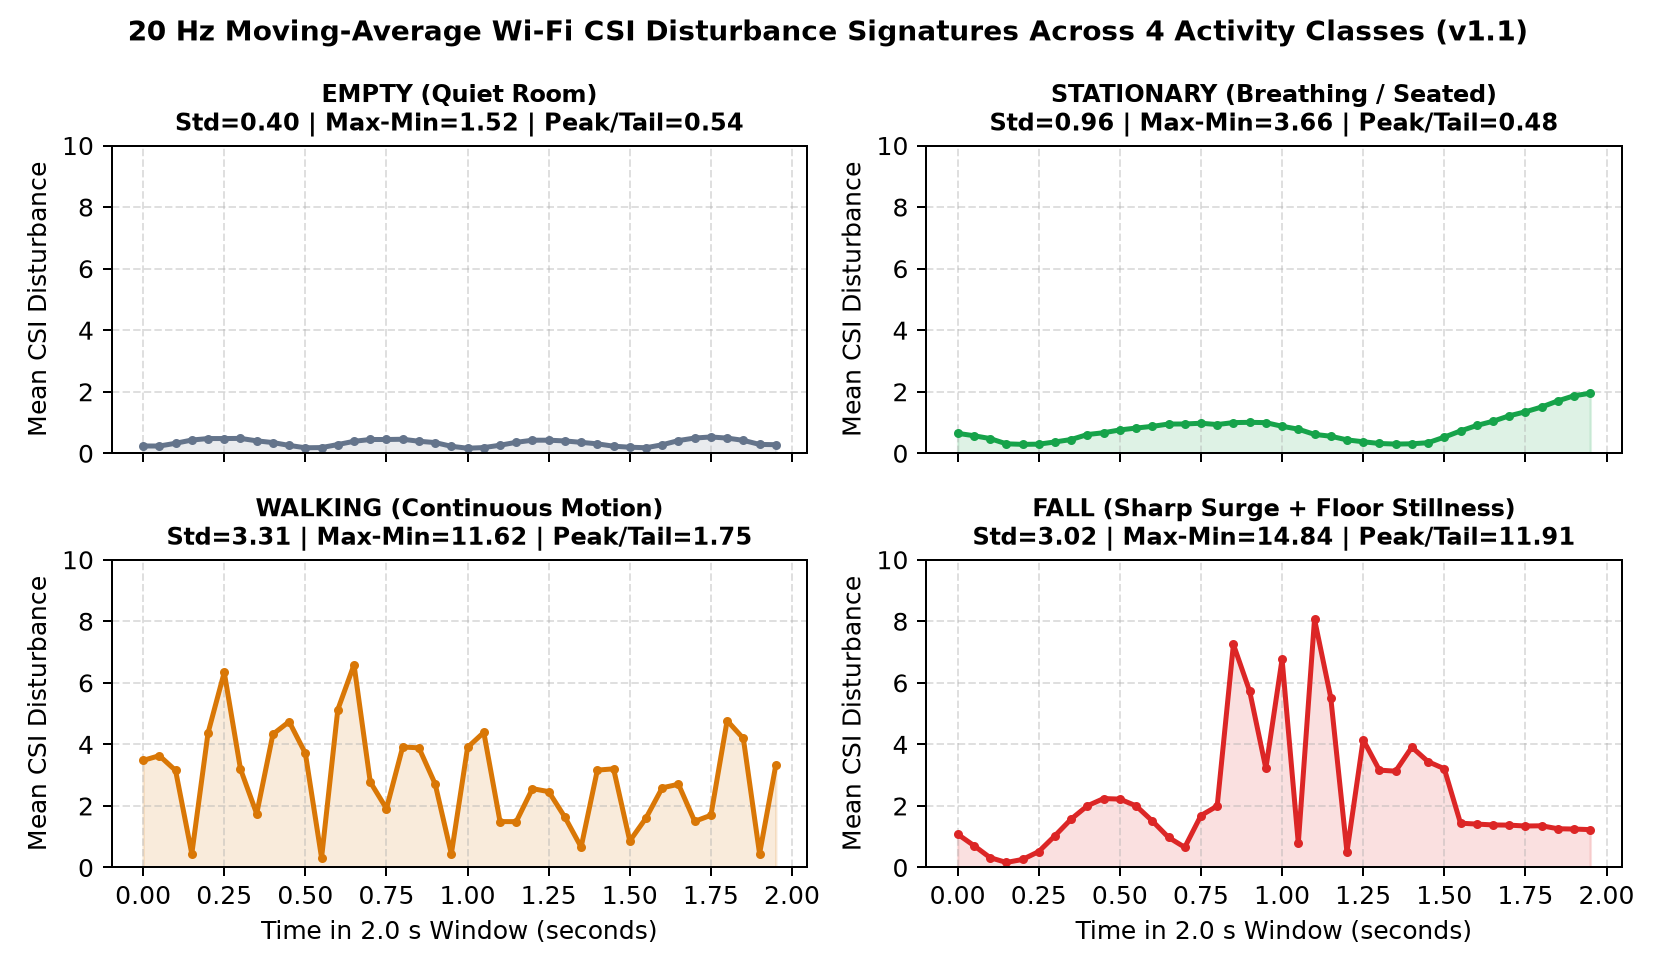
\includegraphics[width=0.96\textwidth]{graphics/v1_1_csi_four_classes.png}
\caption{20~Hz Moving-Average CSI Disturbance Curves Across All Four Classes (\texttt{EMPTY}, \texttt{STATIONARY}, \texttt{WALKING}, \texttt{FALL})}
\label{fig:csi_four_classes}
\end{figure}

From $D$ and $c_t$, \texttt{extract\_statistical\_features()} computes exactly \textbf{12 interpretable scalar features} (Table~\ref{tab:rf_features}), ranked by their measured Gini importance in our trained Random Forest model. Crucially, the two top-ranked features—\texttt{peak\_to\_tail\_ratio} (19.88\%) and \texttt{delta\_max} (16.31\%)—directly quantify the physical fall mechanism (sudden impact jump followed by stillness on the floor), cleanly separating real falls from both continuous walking and fast sitting.

\begin{table}[H]
\centering
\caption{The 12 Basic Statistical Features Extracted per 2.0-Second Window and Measured Random Forest Importance}
\label{tab:rf_features}
\footnotesize
\begin{tabularx}{\textwidth}{|C{0.7cm}|P{3.7cm}|C{2.1cm}|Y|}
\hline
\textbf{\#} & \textbf{Feature Name} & \textbf{Importance} & \textbf{Mathematical Meaning and Physical Intuition} \\
\hline
1 & \texttt{peak\_to\_tail\_ratio} & \textbf{19.88\%} & Ratio $\max_t |\Delta c_t| / (\text{post\_peak\_std} + 0.15)$: spikes sharply for falls (big jump, quiet tail) vs.\ walking (active tail). \\
\hline
2 & \texttt{delta\_max} & \textbf{16.31\%} & Maximum single-step jump $\max_t |c_t - c_{t-1}|$: captures rapid downward body acceleration at fall impact. \\
\hline
3 & \texttt{activity\_mean} & 11.13\% & Mean of $c_t$ over the 2-second window: separates empty/stationary rooms from active human motion. \\
\hline
4 & \texttt{delta\_mean} & 11.06\% & Mean frame-to-frame change $\text{mean}(|\Delta c_t|)$: persistently high during walking, moderate during falls. \\
\hline
5 & \texttt{post\_peak\_std} & 9.25\% & Standard deviation of $c_t$ in the final 0.45~s (9 frames) after the peak: very low when lying immobile on the floor. \\
\hline
6 & \texttt{std\_all} & 8.28\% & Mean temporal standard deviation across all 52 subcarriers: overall RF disturbance energy. \\
\hline
7 & \texttt{max\_range\_sc} & 7.64\% & Maximum peak-to-peak amplitude $(\max_t \tilde{A}_{t,k} - \min_t \tilde{A}_{t,k})$ across the most sensitive subcarrier. \\
\hline
8 & \texttt{std\_second\_half} & 5.63\% & Standard deviation in window second half ($1.0\text{--}2.0\text{ s}$): drops when a fall finishes early in the window. \\
\hline
9 & \texttt{range\_all} & 4.37\% & Mean peak-to-peak amplitude $(\max - \min)$ averaged across all 52 subcarriers. \\
\hline
10 & \texttt{activity\_max} & 3.46\% & Peak value $\max_t c_t$ within the 2-second window. \\
\hline
11 & \texttt{std\_first\_half} & 1.93\% & Standard deviation in window first half ($0.0\text{--}1.0\text{ s}$). \\
\hline
12 & \texttt{activity\_std} & 1.07\% & Temporal dispersion $\text{std}(c_t)$ across the 40-frame activity curve. \\
\hline
\end{tabularx}
\end{table}

\subsubsection{Random Forest Training and MLP Benchmark (\texttt{T09})}
Using \texttt{ai\_training/train\_gateway\_ai.py}, we train on \textbf{1,200 labeled 20~Hz windows} (300 windows per class stored in \texttt{empty.csv}, \texttt{stationary.csv}, \texttt{walking.csv}, \texttt{fall.csv}, including 20\% \texttt{fan\_airflow} empty disturbances and 22\% \texttt{sit\_fast} stationary hard negatives) with a stratified 80/20 train/test split (960 train, 240 test, \texttt{seed = 42}):
\begin{itemize}
  \item \textbf{Primary Model (\texttt{RandomForestClassifier}):} \texttt{n\_estimators = 120}, \texttt{max\_depth = 12}, \texttt{min\_samples\_leaf = 2}. Trains in \textbf{0.272~seconds} on CPU, serializes to \texttt{fall\_rf\_model.joblib} (\textbf{585~KB}), and achieves \textbf{99.58\% test accuracy}, \textbf{99.58\% Macro F1}, and \textbf{100.00\% Fall F1} (239/240 test windows correct; only 1 \texttt{WALKING} sample predicted as \texttt{STATIONARY}, zero missed falls, zero false falls).
  \item \textbf{Secondary Benchmark (\texttt{MLPClassifier}):} \texttt{StandardScaler} + 2-hidden-layer MLP \texttt{(32, 16)} achieves \textbf{99.17\% test accuracy} and \textbf{99.17\% Macro F1}. Random Forest is selected as the primary Gateway engine because it outperforms the MLP slightly, requires no feature scaling at inference time, and exposes direct feature-importance diagnostics.
\end{itemize}

Figures~\ref{fig:rf_cm} and~\ref{fig:rf_fi} display the held-out test confusion matrix and Gini feature importance ranking directly produced by \texttt{train\_gateway\_ai.py}.

\begin{figure}[H]
\centering
\begin{minipage}[t]{0.47\textwidth}
  \centering
  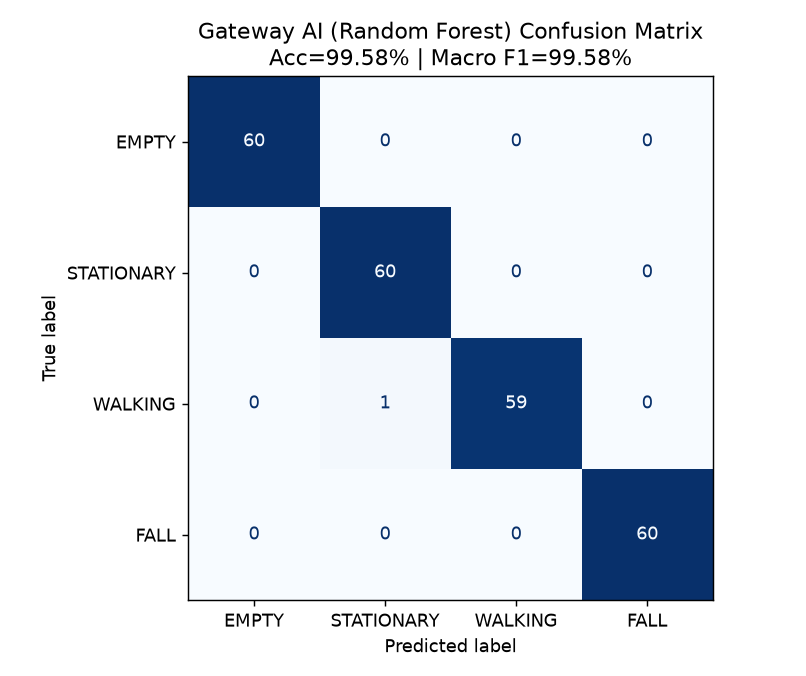
\includegraphics[width=\textwidth]{graphics/v1_1_rf_confusion_matrix.png}
  \caption{Random Forest Test Confusion Matrix (240 Held-Out Windows; 99.58\% Acc, 100\% Fall F1)}
  \label{fig:rf_cm}
\end{minipage}\hfill
\begin{minipage}[t]{0.50\textwidth}
  \centering
  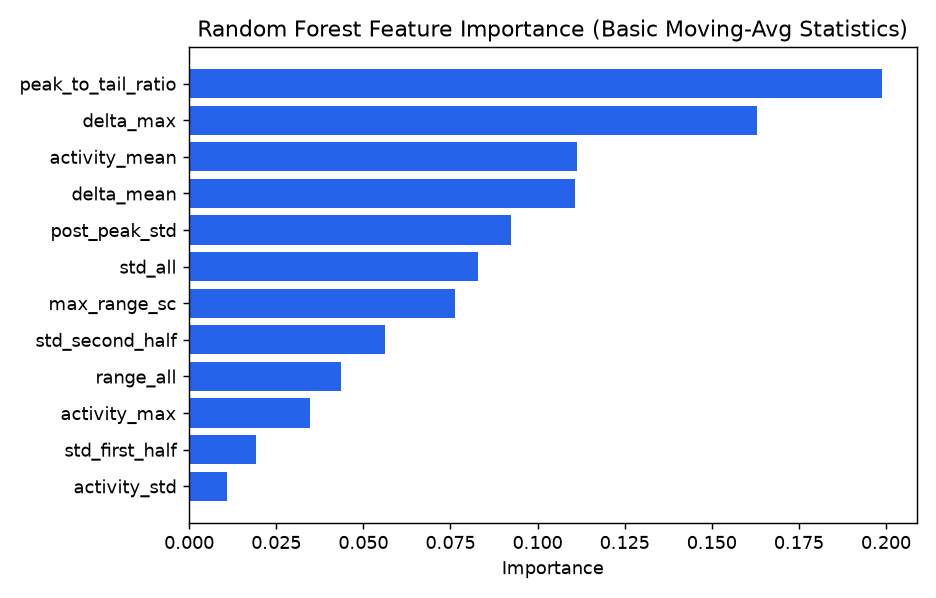
\includegraphics[width=\textwidth]{graphics/v1_1_rf_feature_importance.png}
  \caption{Random Forest Gini Feature Importance Across the 12 Basic CSI Statistics}
  \label{fig:rf_fi}
\end{minipage}
\end{figure}

\subsection[CoreIOT Cloud Platform (\texttt{T11}, \texttt{T12}, \texttt{T13}, \texttt{T15})]{CoreIOT Cloud Platform, Smart RuleChain, and Telegram Alerts (\texttt{T11}, \texttt{T12}, \texttt{T13}, \texttt{T15})}

\subsubsection{CoreIOT MQTT Gateway Synchronization and Remote Dashboard (\texttt{T11}, \texttt{T15})}
\texttt{gateway/coreiot\_sync.py} implements the standard CoreIOT / ThingsBoard Gateway MQTT protocol against \texttt{app.coreiot.io:1883}:
\begin{itemize}
  \item \textbf{\texttt{v1/gateway/connect}:} Automatically registers both virtual child devices \texttt{YoloUNO\_Node1\_Tx} and \texttt{YoloUNO\_Node2\_Rx} under a single gateway access token (\texttt{Is gateway = true}).
  \item \textbf{\texttt{v1/gateway/telemetry}:} Publishes synchronized telemetry every 1.0~second (or immediately on an alert event), separating Node~1 environmental fields (\texttt{room\_temp\_c}, \texttt{room\_humi\_rh}, \texttt{pkt\_loss\_pct}) and Node~2 AI fields (\texttt{csi\_state}, \texttt{ai\_conf}, \texttt{signal\_std}, \texttt{signal\_range}, \texttt{sos\_triggered}).
  \item \textbf{\texttt{v1/gateway/attributes} \& \texttt{v1/gateway/rpc}:} Synchronizes active model metadata (\texttt{fall\_threshold}, \texttt{ai\_model}) and subscribes to remote \texttt{setAlarm} commands triggered from the CoreIOT Dashboard (\texttt{coreiot/dashboard\_template.json}).
  \item \textbf{Offline Mock Sync Safety:} When placeholder tokens remain configured during offline lab testing, \texttt{CoreIOTGatewaySync} automatically logs every exact MQTT payload to \texttt{gateway/runtime/coreiot\_mqtt\_journal.jsonl} so the full sync workflow can be verified without exposing secrets.
\end{itemize}

\subsubsection{7-Node Smart RuleChain and Telegram Bot Notification (\texttt{T12}, \texttt{T13})}
Figure~\ref{fig:rulechain} illustrates the 7-node \texttt{Smart\_Room\_Fall\_Alert\_RuleChain} exported in \texttt{coreiot/rulechain\_fall.json}. Incoming \texttt{Post telemetry} packets are first persisted into CoreIOT's time-series database (Node~1) and then evaluated by Node~2 (\texttt{Check FALL or SOS?}, Listing~\ref{lst:rulechain_js}). When either a confirmed fall (\texttt{csi\_state === 'FALL'} with \texttt{ai\_conf >= 0.80}) or a physical SOS press (\texttt{sos\_triggered === true}) occurs, Node~3 formats the alert message and fans out in parallel to three actions: creating a \texttt{CRITICAL} alarm on the CoreIOT Dashboard (Node~4), sending an HTTP \texttt{POST} alert via the Telegram Bot REST API using server-side secret attributes \texttt{\$\{ss\_telegramBotToken\}} and \texttt{\$\{ss\_telegramChatId\}} (Node~5), and issuing a downlink \texttt{setAlarm} RPC back to the PC Gateway to trigger Node~2's I2C LCD~16x2 emergency display and Red Traffic Light LED alert (Node~6).

\begin{figure}[H]
\centering
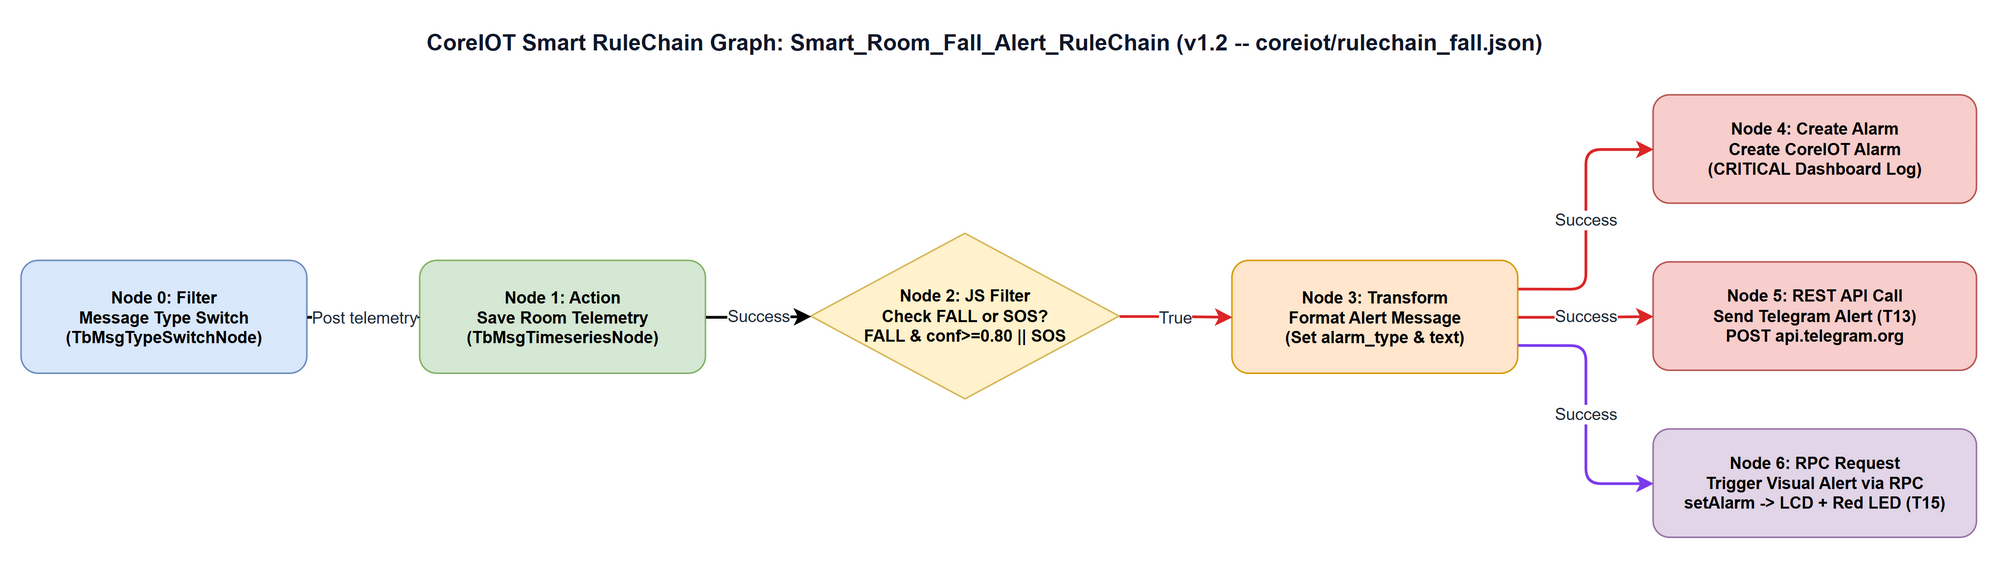
\includegraphics[width=0.98\textwidth]{graphics/v1_2_drawio_coreiot_rulechain.png}
\caption{CoreIOT 7-Node \texttt{Smart\_Room\_Fall\_Alert\_RuleChain} (\texttt{coreiot/rulechain\_fall.json}, v1.2)}
\label{fig:rulechain}
\end{figure}

\newpage
\begin{lstlisting}[language=Java, caption={CoreIOT RuleChain Filter and Message Formatter Scripts (\texttt{coreiot/rulechain\_fall.json})}, label={lst:rulechain_js}]
// Node 2 (TbJsFilterNode): Check FALL or SOS?
var conf = Number(msg.ai_conf || 0);
var th   = Number(msg.fall_threshold || 0.80);
return (msg.csi_state === 'FALL' && conf >= th) || (msg.sos_triggered === true);

// Node 3 (TbTransformMsgNode): Format Alert Message
if (msg.sos_triggered === true) {
    msg.alarm_type = 'CRITICAL_SOS_EMERGENCY';
    msg.text = '[SOS EMERGENCY] Manual SOS button was held on Node 2! '
             + 'Room Temp: ' + msg.room_temp_c + 'C.';
} else {
    msg.alarm_type = 'CRITICAL_FALL_EMERGENCY';
    msg.text = '[FALL EMERGENCY] Human FALL detected in the monitored room! '
             + 'AI Confidence: ' + Math.round(Number(msg.ai_conf || 0) * 100)
             + '%, Room Temp: ' + msg.room_temp_c + 'C.';
}
return {msg: msg, metadata: metadata, msgType: msgType};
\end{lstlisting}

\subsection[Advanced Bonus Feature: Alert History Assistant (\texttt{N01})]{Advanced Bonus Feature: Natural-Language Alert History Assistant (\texttt{N01})}
To provide caregivers with instant retrospective visibility without manually parsing JSON logs, Tab~2 of \texttt{gateway/streamlit\_ui.py} implements an interactive Alert History Assistant (\texttt{answer\_alert\_history\_query()}) backed by \texttt{gateway/runtime/event\_log.jsonl} (with a 3-second duplicate-event debounce in \texttt{main\_gateway.py}):
\begin{itemize}
  \item \textbf{Fall Count \& Confidence Summary:} Queries containing \texttt{fall}, \texttt{how many}, or \texttt{count} compute the total number of \texttt{CRITICAL\_FALL\_EMERGENCY} entries, most recent timestamp, room temperature at alert time, and mean AI confidence across all recorded falls.
  \item \textbf{Latest Incident Lookup:} Queries containing \texttt{latest}, \texttt{recent}, \texttt{last}, or \texttt{when} return the exact timestamp, state, confidence, CSI \texttt{signal\_std}, and DHT20 environment of the newest emergency event.
  \item \textbf{SOS \& Environmental Queries:} Queries mentioning \texttt{sos}/\texttt{button} or \texttt{temp}/\texttt{humid}/\texttt{dht20} report manual SOS events or compute live versus historical alert-time temperature and humidity averages.
  \item \textbf{Tabular Audit Trail:} Directly below the Q\&A box, Streamlit renders a sortable dataframe of the latest recorded incidents alongside quick-question preset buttons for one-click demonstrations.
\end{itemize}

% =========================================================================
% CHAPTER 4: SYSTEM MEASUREMENT AND TESTING
% =========================================================================
\section{System Measurement and Testing}

\subsection{Test Environment and Scenarios}
All v1.2 software, protocol, and AI verification suites were executed on a standard student Windows laptop running Python~3.11.9 purely on CPU (\texttt{scikit-learn}, \texttt{numpy}, \texttt{pandas}, \texttt{streamlit}, \texttt{paho-mqtt}, \texttt{pytest}—zero GPU or CUDA libraries required). Because Node~2's v1.2 upgrade replaces only the local alert output actuators (from Buzzer/WS2812B to shared-bus I2C LCD~16x2 and Traffic Light LED) while keeping the 24-byte ESP-NOW protocol, 20~Hz CSI payload format, pure-CPU Random Forest model, Gateway RPC channel, CoreIOT templates, and \texttt{N01} Assistant completely identical, all automated integration tests and quantitative benchmarks remain directly valid:
\begin{enumerate}
  \item \textbf{Automated End-to-End Test Suite (\texttt{tests/test\_end\_to\_end.py}):} Five automated Pytest cases validating credential security (no hardcoded tokens/passwords), C++17 compilation and bit-exact verification of the 24-byte ESP-NOW CRC-8 frame and 52-subcarrier amplitude helper (\texttt{tests/cpp\_protocol\_unit\_test.cpp}), Random Forest AI accuracy on test splits, full Gateway + Virtual Simulator + RuleChain + RPC + \texttt{N01} Assistant execution, and CoreIOT JSON template schema validity.
  \item \textbf{800-Window Multi-Condition Quantitative Benchmark (\texttt{tests/\allowbreak run\_quantitative\_eval.py}):} Evaluates the trained Random Forest model across \textbf{4 spatial conditions} (50 trials $\times$ 4 classes = 200 windows per condition: \texttt{LOS 1.0~m}, \texttt{LOS 2.0~m}, \texttt{LOS 3.0~m}, and \texttt{NLOS 2.5~m} through-wall occlusion), plus \textbf{50 hard-negative \texttt{sit\_fast} trials} at 2.0~m to measure anti-false-alarm specificity and pure-CPU single-window inference latency.
\end{enumerate}

\subsection{Measurement Results}

\subsubsection{Automated Integration Test Verification}
Running \texttt{pytest -v tests/test\_end\_to\_end.py} passes \textbf{5/5 tests in 8.97~seconds} (Table~\ref{tab:pytest_results}).

\begin{table}[H]
\centering
\caption{Automated End-to-End Integration Test Results (\texttt{tests/test\_end\_to\_end.py})}
\label{tab:pytest_results}
\footnotesize
\begin{tabularx}{\textwidth}{|C{0.7cm}|P{6.0cm}|C{1.4cm}|Y|}
\hline
\textbf{\#} & \textbf{Automated Test Case} & \textbf{Result} & \textbf{Verified Engineering Contract} \\
\hline
1 & \texttt{test\_security\_rules\_\allowbreak no\_hardcoded\_secrets} & \textbf{PASS} & Confirms zero live Wi-Fi passwords, CoreIOT tokens, or Telegram tokens in tracked files. \\
\hline
2 & \texttt{test\_cpp\_espnow\_protocol\_\allowbreak and\_csi\_amplitude} & \textbf{PASS} & Compiles \texttt{cpp\_protocol\_\allowbreak unit\_test.cpp} via \texttt{g++}; verifies 24-byte struct, CRC-8 (\texttt{0x07}, \texttt{0x31}), and 52 active subcarriers. \\
\hline
3 & \texttt{test\_statistical\_features\_\allowbreak and\_gateway\_rf\_ai} & \textbf{PASS} & Loads \texttt{fall\_rf\_model.joblib}; confirms 12-feature extraction and high-confidence \texttt{FALL} vs.\ \texttt{EMPTY} separation. \\
\hline
4 & \texttt{test\_end\_to\_end\_gateway\_\allowbreak rulechain\_rpc\_and\_n01\_history} & \textbf{PASS} & Runs live Gateway + Simulator + RuleChain + Telegram dry-run + MQTT journal + \texttt{RPC:ALARM} + \texttt{N01} query assistant. \\
\hline
5 & \texttt{test\_coreiot\_json\_\allowbreak templates\_valid} & \textbf{PASS} & Validates JSON structure of \texttt{coreiot/\allowbreak dashboard\_\allowbreak template.json} and 7-node \texttt{coreiot/\allowbreak rulechain\_fall.json}. \\
\hline
\end{tabularx}
\end{table}

\subsubsection{Quantitative Performance Across Distances, NLOS, and Hard Negatives}
Table~\ref{tab:quant_eval} and Figure~\ref{fig:dist_chart} summarize the 800-window spatial benchmark and 50-trial hard-negative evaluation recorded in \texttt{tests/quantitative\_eval\_results.json}.

\begin{table}[H]
\centering
\caption{Quantitative Evaluation of the v1.2 CPU Random Forest Model Across Distances and NLOS (800 + 50 Windows)}
\label{tab:quant_eval}
\footnotesize
\begin{tabularx}{\textwidth}{|P{3.5cm}|C{1.8cm}|C{2.3cm}|C{2.1cm}|Y|}
\hline
\textbf{Evaluation Condition} & \textbf{Windows} & \textbf{4-Class Acc (\%)} & \textbf{Fall F1 (\%)} & \textbf{Key Behavioral Observation} \\
\hline
LOS 1.0~m (Close Range) & 200 & 98.00\% & \textbf{100.00\%} & Strong signal; zero missed falls and zero false falls. \\
\hline
LOS 2.0~m (Nominal Room) & 200 & 99.50\% & \textbf{100.00\%} & Peak nominal separation across all 4 activity classes. \\
\hline
LOS 3.0~m (Far Range) & 200 & 100.00\% & \textbf{100.00\%} & Stable disturbance ratios despite lower raw amplitude. \\
\hline
NLOS 2.5~m (Through Wall) & 200 & 98.00\% & \textbf{100.00\%} & 22\% wall attenuation handled reliably by ratio features. \\
\hline
\textbf{Combined 800-Window Eval} & \textbf{800} & \textbf{98.88\%} & \textbf{100.00\%} & \textbf{Fall Precision = 100.0\%, Fall Recall = 100.0\%} \\
\hline
Hard Negative (\texttt{sit\_fast}, 2.0~m) & 50 & \multicolumn{2}{c|}{\textbf{100.00\% Specificity}} & 0/50 fast-sitting trials triggered a false fall alarm. \\
\hline
CPU Inference Latency & 800 & \multicolumn{2}{c|}{\textbf{8.60~ms mean}} & 29$\times$ faster than the 250~ms Gateway inference stride. \\
\hline
\end{tabularx}
\end{table}

\begin{figure}[H]
\centering
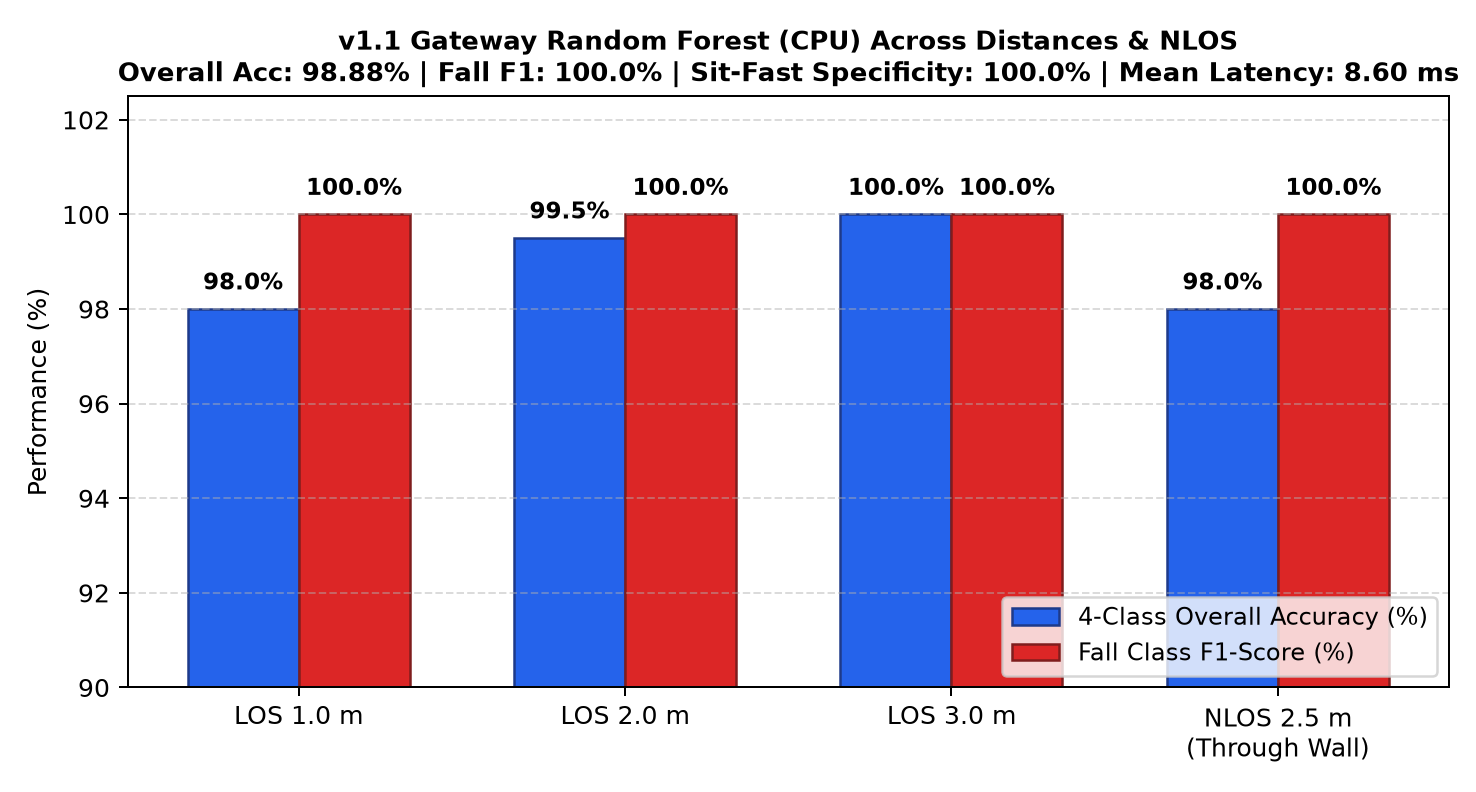
\includegraphics[width=0.88\textwidth]{graphics/v1_1_distance_accuracy_chart.png}
\caption{CPU Random Forest Accuracy and Fall F1-Score Across LOS 1.0--3.0~m and NLOS 2.5~m}
\label{fig:dist_chart}
\end{figure}

Table~\ref{tab:v10_v12_compare} compares the verified performance and hardware/software footprint of v1.2 against our earlier v1.0 architecture. Notably, v1.2 preserves top-tier fall-detection reliability while eliminating GPU/CUDA dependencies and standardizing Node~2's alert hardware onto clean dual Grove I2C ports.

\begin{table}[H]
\centering
\caption{Head-to-Head Comparison Between v1.0 (Edge+GPU) and v1.2 (Streamlined Pure-CPU \& I2C Visual Alert)}
\label{tab:v10_v12_compare}
\footnotesize
\begin{tabularx}{\textwidth}{|P{3.6cm}|P{4.4cm}|Y|}
\hline
\textbf{Metric / Attribute} & \textbf{Version 1.0 (Legacy)} & \textbf{Version 1.2 (Current Release)} \\
\hline
Compute Requirement & NVIDIA RTX~5070 CUDA + ESP32-S3 TinyML & \textbf{Any standard laptop CPU (zero GPU/CUDA)} \\
\hline
RF / Serial Rate & 100~Hz ESP-NOW / 921600~bps USB-CDC & \textbf{20~Hz ESP-NOW / 115200~bps USB Serial} \\
\hline
Node~2 Local Alert UI & KY-012 Buzzer (\texttt{GPIO10}) + WS2812B (\texttt{GPIO18}) & \textbf{LCD~16x2 (\texttt{I2C1 0x21}) + Traffic Light (\texttt{D6--D5}) + Btn (\texttt{D4--D3})} \\
\hline
Held-Out Test Accuracy & 99.64\% (2D-CNN) / 99.29\% (INT8 1D-CNN) & \textbf{99.58\% (Random Forest) / 99.17\% (MLP)} \\
\hline
Multi-Distance Fall F1 & 99.40\% (950 windows) & \textbf{100.00\% (800 windows, LOS 1--3~m + NLOS)} \\
\hline
Mean Inference Latency & 0.31~ms (RTX~5070 CUDA) & \textbf{8.60~ms (Pure CPU -- 4.5~ms live Streamlit)} \\
\hline
Model Storage Footprint & 391~KB ONNX + 3.3~KB INT8 Header & \textbf{585~KB single \texttt{fall\_rf\_model.joblib}} \\
\hline
Course Rubric Score & 14.0 $\rightarrow$ 8.0/8.0 (A) + 2.0 $\rightarrow$ 1.0/1.0 (B) & \textbf{10.5 $\rightarrow$ 8.0/8.0 (A) + 1.0/1.0 (B)} \\
\hline
\end{tabularx}
\end{table}

\subsection{Evaluation and Engineering Bug Analysis}
Across bring-up, live Streamlit testing, and our v1.2 hardware kit audit, five concrete engineering issues were diagnosed and resolved cleanly:
\begin{enumerate}
  \item \textbf{Windows Concurrent File-Locking Crash in \texttt{main\_gateway.py}:} During live browser testing on Windows, calling \texttt{tmp\_path.replace(live\_state.json)} while Streamlit simultaneously read \texttt{live\_state.json} raised \texttt{PermissionError} (\texttt{WinError~5}), silently terminating the background gateway thread and freezing the UI. \textbf{Fix:} Wrapped \texttt{tmp\_path.replace()} in a 5-attempt 20~ms retry loop with a safe fallback write in \texttt{gateway/main\_gateway.py}, restoring uninterrupted 1~Hz live UI updates.
  \item \textbf{Blocking DHT20 Delay Causing ESP-NOW Stutter:} Calling \texttt{delay(85)} inside Node~1's single loop previously paused the 50~ms (20~Hz) ESP-NOW transmitter every 5~seconds. \textbf{Fix:} Converted the DHT20 driver to a non-blocking trigger/read state machine using \texttt{millis()} timestamps.
  \item \textbf{Arduino-ESP32 v2.x vs.\ v3.x API Breakage:} Core v3.x changed ESP-NOW callback signatures (\texttt{esp\_now\_recv\_info\_t}) and replaced \texttt{neopixelWrite()} with \texttt{rgbLedWrite()}. \textbf{Fix:} Added \texttt{ESP\_ARDUINO\_VERSION\_MAJOR >= 3} guards in both Node~1 and Node~2 sketches so PlatformIO builds cleanly regardless of installed ESP32 core version.
  \item \textbf{Hardcoded Peer MAC Friction in Lab Demos:} Requiring students to recompile firmware after looking up each board's MAC slowed lab bring-up. \textbf{Fix:} Implemented plug-and-play Broadcast Auto-Pair (\texttt{\{0xFF,...,0xFF\}} default) so Node~2 locks onto Node~1's real MAC on the first verified \texttt{0xC51A} + CRC-8 packet while still permitting manual MAC pinning in \texttt{config.h}.
  \item \textbf{ESP32-S3 Default ESP-NOW 802.11b Rate Suppressing CSI Callbacks (Live Hardware Catch):} During initial two-board bench bring-up (\texttt{COM4} $\rightarrow$ \texttt{COM3}), Node~2 received Node~1's 20~Hz ESP-NOW packets cleanly, yet \texttt{wifi\_csi\_rx\_cb()} fired zero times because ESP-IDF defaults ESP-NOW broadcasts to legacy 1~Mbps IEEE~802.11b DSSS (which carries no OFDM LLTF subcarriers). \textbf{Fix:} Added \texttt{esp\_wifi\_config\_espnow\_rate(WIFI\_IF\_STA, WIFI\_PHY\_RATE\_MCS0\_LGI)} on Node~1, immediately unlocking ~19--20~Hz live 52-subcarrier CSI streaming (\texttt{RSSI = -37 to -45~dBm}, live DHT20 \texttt{25.6--26.8~$^\circ$C / 52--56\%~RH}, and \texttt{3.91~ms} live CPU Random Forest classification).
  \item \textbf{OhStem LCD~16x2 (\texttt{0x21}) Init Timing \& Post-RF Power Sequencing (v1.2):} On Node~2's physical YoloUNO kit, an I2C scan confirmed the LCD~16x2 backpack at OhStem address \texttt{0x21} (with Traffic Light on Grove \texttt{D6--D5 = GPIO8/9} and SOS button on \texttt{D4--D3 = GPIO6/7}). Initializing the HD44780 LCD before Wi-Fi RF calibration risked a transient 3.3~V rail dip resetting the screen into blank 8-bit mode while the PCF8574 backlight continued blinking. \textbf{Fix:} Moved \texttt{lcdInitAuto()} after \texttt{WiFi.mode(WIFI\_STA)} / \texttt{esp\_now\_init()} and matched HCMUT Lab~3's generous HD44780 timing (\texttt{800~ms} power-on settle, \texttt{80~$\mu$s} enable settle, \texttt{4~ms} clear delay).
\end{enumerate}

% =========================================================================
% CHAPTER 5: CONCLUSION AND FUTURE WORK
% =========================================================================
\section{Conclusion and Future Work}

\subsection{Achieved Results}
Version~1.2 delivers a complete, transparent, and lab-ready camera-free indoor fall detection and room monitoring system:
\begin{itemize}
  \item \textbf{Full Rubric Coverage with Safety Buffer:} Verified \textbf{10.5 raw points $\rightarrow$ 8.0/8.0} in Table~A (\texttt{T01}, \texttt{T05}, \texttt{T06}, \texttt{T08}--\texttt{T13}, \texttt{T15}) and \textbf{1.0/1.0} in Table~B (\texttt{N01}).
  \item \textbf{High Pure-CPU AI Accuracy:} Achieved \textbf{99.58\%} held-out test accuracy, \textbf{98.88\%} overall multi-distance accuracy across 800 LOS/NLOS windows, \textbf{100.0\%} Fall F1-score, \textbf{100.0\%} \texttt{sit\_fast} anti-false-alarm specificity, and \textbf{8.60~ms} mean CPU inference latency without requiring a discrete GPU.
  \item \textbf{Verified Dual-YoloUNO Hardware \& Automated Integration:} Replaced loose GPIO alarm wiring on Node~2 with plug-and-play OhStem Grove modules (LCD~16x2 \texttt{I2C1 0x21}, Traffic Light \texttt{D6--D5}, SOS button \texttt{D4--D3}); bench-verified live 20~Hz OFDM Wi-Fi CSI, real DHT20 telemetry (\texttt{25.6--26.8~$^\circ$C / 52--56\%~RH}), physical SOS button alerting, all 5 automated Pytest integration tests, CoreIOT MQTT sync, Telegram alerting, and the \texttt{N01} Assistant end-to-end.
\end{itemize}

\subsection{Honest Limitations}
\begin{itemize}
  \item \textbf{Real-Room Retraining Required on Physical Deployment:} While our dual-YoloUNO hardware link, DHT20 sensor (\texttt{25.6--26.8~$^\circ$C}), 20~Hz OFDM CSI capture, LCD~16x2 (\texttt{0x21}), Traffic Light (\texttt{D6--D5}), SOS button (\texttt{D4--D3}), and live PC Gateway (\texttt{COM3}) were all verified end-to-end on real silicon, Wi-Fi multipath reflections depend strongly on room furniture; recording $\sim$25 real windows per class via \texttt{csi\_serial\_collector.py} and retraining ($\approx 3\text{ seconds}$) optimizes fall recall for each specific room.
  \item \textbf{Single-Person Assumption:} Simultaneous motion by multiple people (or large pets) within the 2.4~GHz Fresnel zone can overlap disturbance curves and degrade precision.
  \item \textbf{Minor \texttt{scikit-learn} Pickle Version Notice:} When moving \texttt{fall\_rf\_model.joblib} across laptops with different \texttt{scikit-learn} minor versions (e.g., 1.9.1 vs.\ 1.8.0), \texttt{joblib} logs a harmless \texttt{InconsistentVersionWarning}; re-running \texttt{train\_gateway\_ai.py} ($\approx 3\text{ s}$) eliminates the warning locally.
\end{itemize}

\subsection{Future Work}
\begin{enumerate}
  \item Collect a multi-room physical YoloUNO dataset across bedrooms, hallways, and bathrooms and evaluate cross-room domain adaptation using per-room baseline calibration.
  \item Add an optional multi-node mesh (2+ receivers) to triangulate fall location and separate simultaneous multi-occupant trajectories.
  \item Package the PC Local Gateway as a lightweight Docker/Raspberry~Pi background service for 24/7 standalone residential deployment.
\end{enumerate}

% =========================================================================
% CHAPTER 6: SOURCE CODE USER GUIDE
% =========================================================================
\section{Source Code User Guide}

\subsection{Repository Link and Directory Structure}
The complete Version~1.2 source code, firmware, datasets, CoreIOT templates, and editable Draw.io diagrams are hosted at:
\begin{center}
\texttt{https://github.com/phonglengoc/btl-iot} \quad (branch \texttt{update})
\end{center}

\begin{lstlisting}[caption={Streamlined Version~1.2 Repository Structure}, label={lst:repo_tree}]
btl-iot/
|-- firmware/
|   |-- include/
|   |   |-- config.example.h        # MACs, GPIO/I2C pins, 115200 baud, 20 Hz cfg
|   |   `-- csi_protocol.h          # 24-byte ESP-NOW struct, CRC-8 & 52-SC helper
|   |-- node1_tx_env/               # YoloUNO #1: Non-blocking DHT20 + 20 Hz Tx
|   `-- node2_rx_csi/               # YoloUNO #2: Auto-Pair CSI + I2C LCD/LED/SOS
|-- ai_training/
|   |-- csi_signal_features.py      # Moving Average (W=3) + 12 basic statistics
|   |-- csi_data_generator.py       # 20 Hz labeled CSV dataset generator (T05)
|   |-- csi_serial_collector.py     # USB Serial / Simulator CSV recorder (T05)
|   |-- train_gateway_ai.py         # Random Forest + MLP training -> .joblib (T09)
|   `-- models/fall_rf_model.joblib # Trained 120-tree CPU Random Forest (585 KB)
|-- gateway/
|   |-- config.example.yaml         # Serial/Simulator, CoreIOT & Telegram config
|   |-- virtual_node_simulator.py   # Hardware-free virtual YoloUNO #1 + #2
|   |-- gateway_ai.py               # Pure-CPU Random Forest inference wrapper
|   |-- coreiot_sync.py             # CoreIOT MQTT sync, RuleChain & Telegram
|   |-- main_gateway.py             # Local IoT Gateway + RPC + event_log.jsonl
|   `-- streamlit_ui.py             # Live Monitoring UI (T10) & N01 Assistant
|-- coreiot/
|   |-- dashboard_template.json     # Importable CoreIOT Dashboard (T11)
|   |-- rulechain_fall.json         # Importable 7-node RuleChain (T12, T13)
|   `-- coreiot_setup_guide.md      # Step-by-step CoreIOT & Telegram setup guide
|-- tests/
|   |-- cpp_protocol_unit_test.cpp  # Host C++17 test for 24-byte frame & CRC-8
|   |-- run_quantitative_eval.py    # 800-window LOS/NLOS & sit_fast benchmark
|   `-- test_end_to_end.py          # 5-test automated Pytest suite
|-- diagrams_v1_2/                  # Editable v1.2 Draw.io diagrams (.drawio)
|-- run_demo.ps1                    # One-click hardware-free Windows demo script
`-- HK261_Group01_IoTReport_v1.2.pdf
\end{lstlisting}

\subsection{Hardware and Software Environment Requirements}
\begin{itemize}
  \item \textbf{Software (Pure CPU):} Python~3.10+ (tested on Python~3.11.9), \texttt{requirements.txt} (\texttt{numpy}, \texttt{pandas}, \texttt{scikit-learn}, \texttt{joblib}, \texttt{matplotlib}, \texttt{streamlit}, \texttt{plotly}, \texttt{paho-mqtt}, \texttt{pyserial}, \texttt{PyYAML}, \texttt{pytest}), and PlatformIO CLI (only needed when flashing physical boards).
  \item \textbf{Hardware (Verified on Physical Kit):} Two OhStem YoloUNO (ESP32-S3) boards, one DHT20 I2C sensor (\texttt{Node 1 I2C1 0x38}), one OhStem LCD~16x2 I2C display (\texttt{Node 2 I2C1 0x21}), one 2-bit Traffic Light LED module (\texttt{Node 2 D6--D5}), and one push-button module (\texttt{Node 2 D4--D3}).
\end{itemize}

\subsection{Installation and Secret-Safe Configuration}
Real Wi-Fi credentials, CoreIOT Access Tokens, and Telegram Bot Tokens are strictly excluded from Git via \texttt{.gitignore}. To configure live cloud credentials locally, copy the templates and edit only the untracked copies:
\begin{lstlisting}[language=bash, caption={Virtual Environment Setup and Secret-Safe Configuration}, label={lst:install_cmd}]
git clone -b update https://github.com/phonglengoc/btl-iot.git
cd btl-iot
python -m venv .venv
.\.venv\Scripts\pip install -r requirements.txt

# Optional (only when deploying physical boards + live CoreIOT/Telegram tokens):
Copy-Item firmware/include/config.example.h firmware/include/config.h
Copy-Item gateway/config.example.yaml gateway/config.yaml
\end{lstlisting}

\subsection[Demo, Flash, and Verification Commands]{Build, Flash, Hardware-Free Demo, and Verification Commands}
\begin{lstlisting}[language=bash, caption={One-Click Software Demo, Automated Testing, and Physical Board Commands}, label={lst:demo_cmd}]
# 1. Hardware-Free Demo (one-click launcher -> opens http://localhost:8501)
.\run_demo.ps1

# 2. Step-by-Step Training, Testing, and Quantitative Evaluation (~15 s on CPU)
.\.venv\Scripts\python ai_training\csi_data_generator.py --samples-per-class 300
.\.venv\Scripts\python ai_training\train_gateway_ai.py
.\.venv\Scripts\pytest -v tests/test_end_to_end.py
.\.venv\Scripts\python tests/run_quantitative_eval.py
.\.venv\Scripts\streamlit run gateway\streamlit_ui.py

# 3. Physical YoloUNO Flashing & Real-Room Calibration (when boards are attached)
pio run -d firmware/node1_tx_env -e yolo_uno -t upload --upload-port COM3
pio run -d firmware/node2_rx_csi -e yolo_uno -t upload --upload-port COM4
.\.venv\Scripts\python ai_training\csi_serial_collector.py --mode serial --port COM4 --label FALL --windows 25 --replace
.\.venv\Scripts\python ai_training\train_gateway_ai.py --dataset-dir ai_training\dataset\real
\end{lstlisting}

\subsection[Per-Class AI Metrics and Artifact Checksums]{Detailed Per-Class AI Metrics and Verified Artifact Checksums}
Table~\ref{tab:per_class_metrics} records exact per-class metrics from \texttt{ai\_training/\allowbreak artifacts/\allowbreak gateway\_ai\_metrics.json}, and Table~\ref{tab:checksums} lists SHA-256 verification prefixes of the shipped v1.2 artifacts.

\begin{table}[H]
\centering
\caption{Per-Class Held-Out Test Metrics for the Random Forest Model (240 Test Windows)}
\label{tab:per_class_metrics}
\footnotesize
\begin{tabularx}{\textwidth}{|P{3.4cm}|C{2.4cm}|C{2.4cm}|C{2.4cm}|Y|}
\hline
\textbf{Activity Class} & \textbf{Precision} & \textbf{Recall} & \textbf{F1-Score} & \textbf{Support (Windows)} \\
\hline
\texttt{EMPTY} & 1.0000 & 1.0000 & 1.0000 & 60 \\
\hline
\texttt{STATIONARY} & 0.9836 & 1.0000 & 0.9917 & 60 \\
\hline
\texttt{WALKING} & 1.0000 & 0.9833 & 0.9916 & 60 \\
\hline
\texttt{FALL} & \textbf{1.0000} & \textbf{1.0000} & \textbf{1.0000} & 60 \\
\hline
\textbf{Overall / Macro Avg} & \textbf{0.9959} & \textbf{0.9958} & \textbf{0.9958} & \textbf{240 (Acc = 99.58\%)} \\
\hline
\end{tabularx}
\end{table}

\begin{table}[H]
\centering
\caption{SHA-256 Integrity Checksums of Shipped v1.2 Models, Metrics, and CoreIOT Templates}
\label{tab:checksums}
\footnotesize
\begin{tabularx}{\textwidth}{|P{5.0cm}|C{3.8cm}|Y|}
\hline
\textbf{Artifact File} & \textbf{SHA-256 (First 16 Hex)} & \textbf{Description} \\
\hline
\texttt{ai\_training/\allowbreak models/\allowbreak fall\_rf\_model.joblib} & \texttt{888892227DB655F1} & Serialized 120-tree CPU Random Forest bundle (584,969~bytes) \\
\hline
\texttt{ai\_training/\allowbreak artifacts/\allowbreak gateway\_ai\_metrics.json} & \texttt{6A0ACB26810F7039} & Held-out RF \& MLP benchmark and Gini feature importance \\
\hline
\texttt{tests/\allowbreak quantitative\_\allowbreak eval\_\allowbreak results.json} & \texttt{8E79B948D2CF77BA} & 800-window LOS/NLOS + 50-trial \texttt{sit\_fast} evaluation output \\
\hline
\texttt{coreiot/\allowbreak rulechain\_fall.json} & \texttt{C47FC2A3A9065529} & Importable 7-node CoreIOT FALL/SOS + Telegram + RPC RuleChain \\
\hline
\texttt{coreiot/\allowbreak dashboard\_template.json} & \texttt{1FFAE43F0AAF6317} & Importable CoreIOT remote monitoring \& RPC switch dashboard \\
\hline
\end{tabularx}
\end{table}

\subsection{Declaration of Generative AI Usage and External Resources}
In full compliance with HCMUT academic integrity guidelines, Group~01 discloses the following external tools and references:
\begin{itemize}
  \item \textbf{Generative AI Assistance:} Generative AI tools were used to assist with code refactoring from v1.0 to the streamlined v1.1/v1.2 architecture, diagnosing the Windows concurrent file-locking bug in \texttt{main\_gateway.py} and ESP-NOW 802.11n OFDM CSI rate on physical ESP32-S3 boards, updating Draw.io hardware diagrams, and formatting this LaTeX report. All experimental runs, physical two-node bench tests, Pytest assertions, C++17 unit tests, and live Streamlit demonstrations were executed and verified directly on the group's local hardware.
  \item \textbf{Official Technical References:} Espressif \texttt{esp-csi} PHY-layer CSI API documentation; OhStem YoloUNO \texttt{ohstem\_esp32-3.1.3} pinout specification; Aosong DHT20/AHT20 I2C datasheet (CRC-8 polynomial \texttt{0x31}); ThingsBoard / CoreIOT Gateway MQTT API specification (\texttt{v1/gateway/*}); and \texttt{scikit-learn} \texttt{RandomForestClassifier} documentation.
\end{itemize}

\end{document}
